% Version 1.2.0 EN
%
%%%%%%%%%%%%%%%%%%%%%%%%%%%%%%%%%%%%%%%%%%%%%%%%%%
%%%        			Preamble!            				   %%%
%%%%%%%%%%%%%%%%%%%%%%%%%%%%%%%%%%%%%%%%%%%%%%%%%%

%%%%%%%%%%%%%%%%%%%%%%%%%%%%%%%%%%%%%%%%%%%%%%%%%%
%%%        		Preamble / compile!       		   %%%
%%%%%%%%%%%%%%%%%%%%%%%%%%%%%%%%%%%%%%%%%%%%%%%%%%

% Important:
% To avoid errors and problems when compiling, please always use the current version of your operating system (Windows / Mac / Linux), the current version of your LaTeX distribution (MiKTeX / MacTeX / Tex Live) and the current version of your typesetting program or LaTeX editor (TeXstudio / Texmaker / TeXworks / TeXnicCenter). Update your operating system, your LaTeX distribution and your LaTeX editor before compiling this template or have them updated by your department IT representative.
%
% Notes on compile / setting order:
% For the correct display of the layout and the bibliographies (multibib) please compile as follows (see "Order of compilation operations"):
%
%- Windows 10: via the PowerShell or command prompt (cmd).
% To do this, go to the folder of this project, do not select any file, click on an empty space with the left mouse button and open the context menu while holding down the Shift key (Shift key + right mouse click) and select "Open PowerShell window here". Then enter "cmd" and call the compile processes individually as follows (see "Order of compilation operations"):
%
%- macOS Big Sur 11.0.1: via the terminal.
% To do this, go to the parent folder of this project and select the folder in which the project is located. Now open the context menu (secondary click) by pressing Control + mouse button or tapping with two fingers on the trackpad. Now select "New Terminal at Folder" and call up the compile processes individually as follows:
%
%
%- Order of compilation operations
% pdflatex KSP_Diss_17x24
% bibtex KSP_Diss_17x24
% bibtex journal				    % The file name of the file to be executed with Bibtex is specified in the command "\ newcites {}" in this TeX file
% bibtex conference				% The file name of the file to be executed with Bibtex is specified in the command "\ newcites {}" in this TeX file
% pdflatex KSP_Diss_17x24
% pdflatex KSP_Diss_17x24
%
%
% Done. 

%%%%%%%%%%%%%%%%%%%%%%%%%%%%%%%%%%%%%%%%%%%%%%%%%%
%%%        			Peamble / Documentclass!       %%%
%%%%%%%%%%%%%%%%%%%%%%%%%%%%%%%%%%%%%%%%%%%%%%%%%%

% Loads the document class "scrbook" (KOMA-Script-Book) with the properties: no dots after the numbering, font size 10pt, language packs: English
\documentclass[%
fontsize=10pt,% Font size 10 points
numbers=noenddot,% No end point after the numbering (i.e. 3.1 instead of 3.1.)
% chapteratlists=0pt,% toc, lot, lof: Set the vertical distance between the entries to 0
toc=listof,% Sets the table of figures (lof) and the table of tables (lot) in the table of contents (toc)
% toc=bibliography,% Places the bibliography in the table of contents (does not work with multiple bibliographies, even if the commands in the file "Contents/Bibliography.tex" are commented out: "\addcontentsline{toc}{section}{Journalartikel}", "\addcontentsline{toc}{section}{Konferenzbeiträge}", "\addcontentsline{toc}{chapter}{Literaturverzeichnis")
toc=chapterentrywithdots,% Adds a dotted line to the page number in the table of contents for headings in the "\chapter" category
% headings=optiontotocandhead,% To use the command "\addchap[tocentry={unnumbered in the table of contents},head={unnumbered in the table of contents}]{unnumbered}{}"
% headinclude,% 
% twoside,% Default for this document class "scrbook"
listof=nochaptergap,% No vertical spacing between the entries (chapter by chapter) in the list of figures or tables
% toc=flat% Reduces the space between the number on the left and text to a minimum; Subchapters are not indented
% toc=chapterentrydots=true,% KOMA guide, p. 74
% toc=sectionentrydots=true% KOMA guide, p. 74
]{scrbook} % Loads the document class "scrbook" (KOMA-Script-Book by Markus Kohm et al.)

%\documentclass[halfparskip,numbers=noenddot,a5paper,10pt,english,ngerman]{scrbook}


% Input, including umlauts (ä, ö, ü and ß) using the parameter [utf8]
\usepackage[utf8]{inputenc}

% Output, including umlauts
\usepackage[T1]{fontenc}

% Load the language packs for hyphenation
\usepackage[english]{babel}

% Insert more packages here
\usepackage{booktabs}
\usepackage{wrapfig}
\usepackage[all]{nowidow} % Prevents widows
\usepackage{amsmath}
\usepackage{amsfonts}
\usepackage{amssymb}
\usepackage{graphicx}
\usepackage[]{acronym}
\usepackage{trfsigns}
\usepackage{caption} % For subfigures
\usepackage{subcaption} % For "subfloat" environments (multi-image graphics / multiple images)
%\usepackage{subfigure} % Old package for "subfigures"
\usepackage{enumitem}
\usepackage{calc}
\usepackage{multirow}
\usepackage{textcmds} % For quotation marks
\usepackage{blindtext} % Enable blind text to display text in the template
\usepackage{fancyvrb} % For Verbatim environments to output LaTeX source code
%\usepackage{showframe} % Show margins
\usepackage{todonotes}
\usepackage{svg}

%%%%%%%%%%%%%%%%%%%%%%%%%%%%%%%%%%%%%%%%%%%%%%%%%%
%%%    		Preamble / Hyphenation!    	     	   %%%
%%%%%%%%%%%%%%%%%%%%%%%%%%%%%%%%%%%%%%%%%%%%%%%%%%

\hyphenation{
Ge-schich-te
An-ten-ne
% Please add words that should not be separated into this list without a hyphen
}

%%%%%%%%%%%%%%%%%%%%%%%%%%%%%%%%%%%%%%%%%%%
%%%    Preamble / Cite!  / Quote!       %%%
%%%%%%%%%%%%%%%%%%%%%%%%%%%%%%%%%%%%%%%%%%%

% Both \citep and \citet are defined by natbib and are thus not standard. The standard LATEX command \cite should be avoided, because it behaves like \citet for author–year citations, but like \citep for numerical ones
% Quoting from the bibliography "Literature.bib": "\citet{<ID>}" respectively "\citep{<ID>}"
% Quoting from the bibliography "Own_journal_papers.bib": "\citetjournal{<ID>}" respectively "\citepjournal{<ID>}"
% Quoting from the bibliography "Own_conference_papers.bib": "\citetconference{<ID>}" respectively "\citepconference{<ID>}"

% Quotation marks
% You form the English introductory quotation marks in LaTeX with two acute accents one after the other, i.e. with the characters `` (shift+´).
% Complete your English quote with two apostrophes in a row. So you write the sign '' (shift+#).

% By default, all titles / references are output in the bibliographies. If only the quoted titles / references are to be output in the bibliography, the command "\nocite{*}" or "\nocitejournal{*} or "\nociteconference{*} "must be commented out in the file "./Inhalt/Literaturverzeichnis.tex"

%\usepackage{cite}
\usepackage[%
round,% (Default) for round parentheses;
%square,% For square brackets
%curly,% For curly braces
%semicolon, % (Default), trennt mehrere Autoren mit Semicolon
%comma, % (Default) to separate multiple citations with semi-colons
%authoryear, % (Default) for author–year citations
%numbers, % For numerical citations
%super, % For superscripted numerical citations, as in Nature
]{natbib}
%
\bibpunct{(}% Left paranthesis
{)}% Right paranthesis
{,}% Separation between several titles in the text
{a}% Citation style: n=for numerical style, s=for numerical superscript style, a=any other letter for author–year, (default) author–year
{}% Punctuation before the year
{,}% Punctuation between different publication years of titles by the same author
%
% Cite!
% The following examples are taken from Patrick W. Daly (2010) "Natural Sciences Citations and References. Author-Year and Numerical Schemes"
%\citet{jon90} --> Jones et al. (1990)
%\citet[chap.~2]{jon90} --> Jones et al. (1990, chap. 2)
%\citep{jon90} --> (Jones et al., 1990)
%\citep[chap.~2]{jon90} --> (Jones et al., 1990, chap. 2)
%\citep[see][]{jon90} --> (see Jones et al., 1990)
%\citep[see][chap.~2]{jon90} --> (see Jones et al., 1990, chap. 2)
%\citet*{jon90} --> Jones, Baker, and Williams (1990)
%\citep*{jon90} --> (Jones, Baker, and Williams, 1990)
%
%\citet{jon90,jam91} --> Jones et al. (1990); James et al. (1991)
%\citep{jon90,jam91} --> (Jones et al., 1990; James et al. 1991)
%\citep{jon90,jon91} --> (Jones et al., 1990, 1991)
%\citep{jon90a,jon90b} --> (Jones et al., 1990a,b)

%%%%%%%%%%%%%%%%%%%%%%%%%%%%%%%%%%%%%%%%%%%%%%%%%%
%%%       Preamble /  Bibliography!            %%%
%%%%%%%%%%%%%%%%%%%%%%%%%%%%%%%%%%%%%%%%%%%%%%%%%%

\usepackage[resetlabels]{multibib} % Each bibliography begins with counter [1], provided that "\ bibliographystyle {plain}" is selected as the bibliography style
\usepackage{multibib} % The bibliographies counter is not reset (counting starting with [1] in "Journal articles" and will be continued in "Conference contributions"), provided that "\ bibliographiestyle {plain}" is selected as the bibliography style, with a different bibliography style, e.g. "\ bibliographystyle {alpha} no counter is used
\newcites{journal}{Bibliography/Own_journal_papers}
\newcites{conference}{Bibliography/Own_conference_papers}
%
\usepackage{etoolbox}
\BeforeBeginEnvironment{thebibliography}{% Redefine to insert your own publications without breaking
  \let\origchapter\chapter % Save the original definition of "\chapter"
  \let\chapter\section % Make \chapter behave like "\section"
}
\AfterEndEnvironment{thebibliography}{%
  \let\chapter\origchapter % Restore the original definition of "\chapter"
}

%%%%%%%%%%%%%%%%%%%%%%%%%%%%%%%%%%%%%%%%%%%%%%%%%%
%%%        Preamble / Title!          		     %%%
%%%%%%%%%%%%%%%%%%%%%%%%%%%%%%%%%%%%%%%%%%%%%%%%%%
\usepackage[scaled]{helvet}
\renewcommand{\familydefault}{\sfdefault}

\usepackage{graphicx,xcolor}
\usepackage{tikz}
\usetikzlibrary{calc}
% PDF-Title
\newcommand{\pdftitle}{Non-Invasive\ Blood\ Glucose\ Monitoring\ in\ Ears}

% Author
\newcommand{\autor}{Andrej\ Vladimirovič\ Ermoshkin}

% Most of the preamble is moved to the "dokOptions.tex" file; The file must be integrated at this point
% Settings such as scaling, font, spacing and the packages "geometry", "figure", "captions" are managed in the following file
% Version 1.2.0 EN
%
% Show page limits to check the page display
%\usepackage{showframe}

%%%%%%%%%%%%%%%%%%%%%%%%%%%%%%%%%%%%%%%%%%%%%%%%%%
%%% 		Manual line break in the 		   %%%
%%%			list of figures and tables		   %%%
%%%%%%%%%%%%%%%%%%%%%%%%%%%%%%%%%%%%%%%%%%%%%%%%%%

% Set line breaks manually in \ listoffigures and \ listoftables with "\ protect \\" (without quotation marks) in the optional parameter of the "\ caption" command
% Example: 
%\caption[Exterior view of the KIT library. Consetetur sadipscing elitr,\protect\\ sed diam nonumy eirmod tempor invidunt ut labore]{Exterior view of the KIT library. Consetetur sadipscing elitr, sed diam nonumy eirmod tempor invidunt ut labore}

%%%%%%%%%%%%%%%%%%%%%%%%%%%%%%%%%%%%%%%%%%%%%%%%%%
%%% 			Special character			  %%%%
%%%%%%%%%%%%%%%%%%%%%%%%%%%%%%%%%%%%%%%%%%%%%%%%%%

% Non-breaking space, protected space: ~
% Non-breaking narrow space, protected narrow space: \.
% Backslash: \textbackslash
% Percent sign: \%
% Ampersand: \&
% Circumflex: \^
% Tilde: \~
% Dollar: \$
% Hashtag, number sign: \#
% Low line: \_
% Curly bracket: \{
% Non-breaking hyphen: "~ % Requires the package "\usepackage[english]{babel}"
% Non-breaking hyphen alternative: \hbox{-}
% Soft hyphen: \-

%%%%%%%%%%%%%%%%%%%%%%%%%%%%%%%%%%%%%%%%%%%%%%%%%%
%%% 			General Settings			  %%%%
%%%%%%%%%%%%%%%%%%%%%%%%%%%%%%%%%%%%%%%%%%%%%%%%%%

% Adjust margins
\setlength{\topskip}{10.5pt} % Prevent an error message

%%%%%%%%%%%%%%%%%%%%%%%%%%%%%%%%%%%%%%%%%%%%%%%%%%
%%%        			Scaling					  %%%%
%%%%%%%%%%%%%%%%%%%%%%%%%%%%%%%%%%%%%%%%%%%%%%%%%%

% Please scale the page margins according to the number of pages in your document (see optional parameters in the following package "\usepackage{geometry}":

% - up to 199 pages ("inner": 20mm, "outer": 15-18mm) >>> textwidth = 113mm
% - 200 to 399 pages ("inner": 23mm, "outer": 15-18mm) >>> textwidth=110mm
% - from 400 pages ("inner": 25mm, "outer": 15mm) >>> textwidth = 108mm

%%%%%%%%%%%%%%%%%%%%%%%%%%%%%%%%%%%%%%%%%%%%%%%%%%
%%%        			Paper size (17x24)		   %%%
%%%%%%%%%%%%%%%%%%%%%%%%%%%%%%%%%%%%%%%%%%%%%%%%%%

% Note: The margins for scaling (see "Scaling" above) can be managed using the "geometry" package, please refer to the corresponding documentation at: http://ftp.fau.de/ctan/macros/latex/contrib/geometry/geometry.pdf

% (DIN 17x24)
\usepackage[%
papersize={17cm,24cm},% Paper size
headheight=1.5\baselineskip,% Line below header
top=25mm,% Distance from the top edge
inner=20mm,% Distance from the inner edge
outer=15mm,% Distance from the outer edge
%lines=38,% Number of lines. It is recommended to comment out because it leads to problems with the correct calculation
%textwidth=113mm,% Width of the type area. It is recommended to comment out because it leads to problems with the correct calculation
footnotesep=7mm,% Vertical distance between the type area and the footnote line
heightrounded=true%
]{geometry}

%%%%%%%%%%%%%%%%%%%%%%%%%%%%%%%%%%%%%%%%%%%%%%%%%%
%%%        				Footer!				   %%%
%%%%%%%%%%%%%%%%%%%%%%%%%%%%%%%%%%%%%%%%%%%%%%%%%%

% Distance between text body (type area) and bottom edge of footer (page numbers)
\setlength{\footskip}{13.6mm}

% Distance between body text and footnote dividing line
\setlength{\skip\footins}{20pt}

%%%%%%%%%%%%%%%%%%%%%%%%%%%%%%%%%%%%%%%%%%%%%%%%%%
%%%        			Footnote!				   %%%
%%%%%%%%%%%%%%%%%%%%%%%%%%%%%%%%%%%%%%%%%%%%%%%%%%

% (1) Position and size of the footnotes for 2-digit footnote numbers
\deffootnote[1.8em]{1.8em}{0em}{\makebox[1.7em][l]{\textsuperscript{\thefootnotemark\ }}}
% \ deffootnote {"Position of the footnote number from the left (and adjust this value)"} {"Indentation of the second line"} {\ makebox ["Distance between the footnote number and the footnote text (and adjust this value)"] [l] {\ thefootnotemark }}

% (2) Please select the following command for 3-digit footnote numbers and deactivate (1) "\ deffootnote {1.7em} {0em} {\ makebox [1.7em] [l] {\ thefootnotemark}}" by comment out the previous command
%\deffootnote{2.2em}{0em}{\makebox[2.2em][l]{\thefootnotemark}}
% \ deffootnote {"Position of the footnote number from the left (and adjust this value)"} {"Indentation of the second line"} {\ makebox ["Distance between the footnote number and the footnote text (and adjust this value)"] [l] {\ thefootnotemark }}

% Prevents footnotes from continuing on the opposite page
\interfootnotelinepenalty=10000 

%%%%%%%%%%%%%%%%%%%%%%%%%%%%%%%%%%%%%%%%%%%%%%%%%%
%%%  				Paragraph!			  	   %%%
%%%%%%%%%%%%%%%%%%%%%%%%%%%%%%%%%%%%%%%%%%%%%%%%%%

% Distribute lines on the page (the lower margin is not compensated by expanding the paragraph spacing)
\raggedbottom   

% Indentation depth (horizontal distance) of the first line of the paragraph
\setlength{\parindent}{0pt}

% Vertical space between paragraphs
\setlength{\parskip}{2.5mm}

% Prevents orphans (single line at the bottom of the page)
\clubpenalty = 10000 

% prevents widows (single line at the top of the page)
\widowpenalty = 10000
\displaywidowpenalty = 10000

% Prevent hyphenation at the page break
\brokenpenalty = 10000

%%%%%%%%%%%%%%%%%%%%%%%%%%%%%%%%%%%%%%%%%%%%%%%%%%
%%%				Caption! 					   %%%
%%%  			Floating objects			   %%%
%%%				Figure!, Table!			   	   %%%
%%%%%%%%%%%%%%%%%%%%%%%%%%%%%%%%%%%%%%%%%%%%%%%%%%

\usepackage[%
labelfont=bf,% Bold text for the designation "Figure" and "Table"
font=footnotesize,% Font size for captions
]{caption}

% Illustrations
\captionsetup[figure]{position=below}
\captionsetup[figure]{aboveskip=3mm} % Distance between image and caption
\captionsetup[figure]{belowskip=-2mm} % Distance between caption and running text

% Tables
% When using "\captionabove" the values "aboveskip" and "belowskip" are swapped; so please use "\caption" for table headings
\captionsetup[table]{position=top}
\captionsetup[table]{aboveskip=0.8mm} % Spacing: running text - table heading (measured in PDF = ~ 7mm) | Note: with the command "\captionabove" the order of the captions changes to: table heading - table
% \captionsetup[table]{aboveskip=1.5mm} % Spacing: running text - table heading (measured in PDF = ~ 7mm) | Note: with the command "\captionabove" the order of the captions changes to: table heading - table
\captionsetup[table]{belowskip=2.5mm} % Spacing: table heading - table (measured in PDF = ~3mm) | Note: with the command "\captionabove" the order of the captions changes to: running text - table heading

% Intextsep! und textfloat!
% Distance illustration: running text - image; caption - running text
% Space table: running text - table heading; table - running text
\setlength{\intextsep}{5.5mm plus0mm minus0mm}% Distance for floating objects placed with the parameter "[h]" (measured in PDF for tables = ~ 8mm; for images = ~ 6mm)
\setlength{\textfloatsep}{7mm plus0mm minus0mm}% Distance for floating objects placed with the parameter "[t]" or "[b]"

% Caption for subfloat!
\captionsetup[subfloat]{%
	labelformat=empty,%
	margin=0pt,% Indentation of the caption from the left
	% skip = 0pt,% Distance between picture and caption
	aboveskip=2mm, % Distance between picture and caption
	belowskip=0mm,% Distance between the caption and the next row of images as well as between the caption and the signature of the figure / since the commands "\captionsetup[subfloat]{belowskip}" and "\captionskip[figure]{skip}" overlap, the vertical distance between the rows of images must be set with the command "\vspace{3mm}"
	% font = {footnotesize, rm},%
	% labelfont = {footnotesize, bf},%
	% format=hang,% Indent second and further lines (align to the first)
	indention=0em,% Indentation of the inscription
	labelsep=space,% "period, space, quad, newline"
	justification = RaggedRight,% Flutter replacement with hyphenation
	% justification = raggedright,% Flutter replacement without hyphenation
	% justification = centering,% Centered
	% justification = justified,% Justification
	singlelinecheck = true,% "false" (true = always center one line)
	position=auto,% "top, bottom"
	labelformat=parens% "simple, empty" = how the label is set
}

%%%%%%%%%%%%%%%%%%%%%%%%%%%%%%%%%%%%%%%%%%%%%%%%%%
%%%  			Floating! objects			   %%%
%%%				"{figure}", "{table}"	   	   %%%
%%%				Layout, size  	   			   %%%
%%%%%%%%%%%%%%%%%%%%%%%%%%%%%%%%%%%%%%%%%%%%%%%%%%

% Minimum fill level of one side with a floating object
\renewcommand{\floatpagefraction}{0.7}

% Maximum size of a floating object at the bottom of the page
\renewcommand{\topfraction}{0.8}

% Maximum size of a floating object at the top of the page
\renewcommand{\bottomfraction}{0.8}

% Possible increase in spacing within a line if the line break is unsightly
\setlength{\emergencystretch}{4pt}

% Minimum amount of text on a page with a floating object
\renewcommand{\textfraction}{0.1}

%%%%%%%%%%%%%%%%%%%%%%%%%%%%%%%%%%%%%%%%%%%%%%%%%%
%%%  				Line spacing!			   %%%
%%%%%%%%%%%%%%%%%%%%%%%%%%%%%%%%%%%%%%%%%%%%%%%%%%

% Set the line spacing to 1
%\usepackage[singlespacing]{setspace}

% Set line spacing to 1.15
\usepackage{setspace}
\setstretch{1.15}

% Set line spacing to 1.2
%\usepackage{setspace}
%\setstretch{1.2}

% Set line spacing to 1.5
%\usepackage[onehalfspacing]{setspace}

%%%%%%%%%%%%%%%%%%%%%%%%%%%%%%%%%%%%%%%%%%%%%%%%%%
%%%				Directories!				   %%%
%%% 			Table of contents	   		   %%%
%%%				Table of figures 			   %%%
%%%				Table of tables 			   %%%
%%%%%%%%%%%%%%%%%%%%%%%%%%%%%%%%%%%%%%%%%%%%%%%%%%

% toc = table of contents 
% lof = list of figures
% lot = list of tables

\makeatletter
%
% Automatic line break in directories (toc, lof, lot) for long headings, horizontal distance to the right margin of the type area; "plus1fil": No hyphenation in the table of contents, this mostly overrides the justification for directories because hyphenation is not possible
\renewcommand\@tocrmarg{8em plus1fil}%new
% \renewcommand\@tocrmarg{7em plus1fil}%new
% \renewcommand\@tocrmarg{4em plus1fil}%old

% Distance between the page number in the table of contents and the last point of the dotted line
\renewcommand\@pnumwidth{1em} % !With 8pt or 0em, sets the page number outside the type area (see "\usepackage{showframe}"!
%
% Changes the distance between the points of the dotted line
% \renewcommand*{\@dotsep}{1.5}% Default ist 4.5
%
% \renewcommand*\l@chapter{\@dottedtocline{0}{1.5em}{2em}}
%
% \renewcommand*\l@figure{\@dottedtocline{1em}{0em}{2.3em}}% Default is {1.5em}{0em}{2.3em}
% \let\l@table\l@figure
%
\makeatother

% Indentation of the chapter number (tocindent) and space between chapter number and chapter text (heading) in the table of contents (tocnumwidth)
\RedeclareSectionCommand[tocindent=0em,tocnumwidth=1.5em]{chapter}
\RedeclareSectionCommand[tocindent=1.5em,tocnumwidth=1.9em]{section}
\RedeclareSectionCommand[tocindent=3.4em,tocnumwidth=2.6em]{subsection}

% List of figures! Indentation and spacing
\DeclareTOCStyleEntry[%
dynnumwidth=true,% If necessary, the spacing of "numsep" is extended (e.g. with two digits)
indent=0pt,% Indentation left
numsep=1em,% Spacing between the number on the left and the text (title of the illustration), maintains the spacing from the page number
numwidth=3em,% Space between number on the left and text (figure title)
% pagenumberbox=1em,% Space between number on the left and text (figure title)
% pagenumberwidth=1em,% Distance between the page number and the text (left), also shifts the dotted line to the left
% listname={Abbildungsverzeichnis},% Name of the list of figures
% pagenumberformat=\sfamily\large,% Page number font
% entryformat=\sffamily\large,% Directory font
rightindent=8em,% Space between page number on the right and text (figure title), hyphenation is active
]{default}{figure}

% List of tables! Indentation and spacing
\DeclareTOCStyleEntry[%
dynnumwidth=true,% If necessary, the spacing of "numsep" is extended (e.g. with two digits)
indent=0pt,% Indentation of the numbering on the left
numsep=1em,% Space between number on the left and text (table title), keeps the space to page number
numwidth=3em,% Space between number on the left and text (table title)
% pagenumberbox=1em,% Space between number on the left and text (table title)
% pagenumberwidth=1em,% Distance between the page number and the text (left), also shifts the dotted line to the left
% beforeskip=1.15em plus 1pt,%
% linefill=\skillmon@chapter@dotfill,%
% entryformat=\textbf%
% pagenumberbox=\relax,%
% listname={Tabellenverezichnis},% Name of the list of tables
% pagenumberformat=\ssfamily\large,% Page number font
% pagenumberformat=\usekomafont{tocentry},% Alternatively
% entryformat=\sffamily\large,% Directory font
rightindent=8em,% Space between page number on the right and text (table title), hyphenation is active
]{default}{table}

% Directory font family (toc, lof, lot)
% \addtokomafont{disposition}{\sffamily} % Font without serifs
% \addtokomafont{disposition}{\rmfamily} % Font with serifs

% Page numbers in the table of contents for headings in the "\chapter" category
\setkomafont{chapterentrypagenumber}{\rmfamily} % Page numbers in the table of contents with serifs
% \setkomafont{chapterentrypagenumber}{\rmfamily\mdseries} % Page numbers in the table of contents in serifs, but not in bold

% \addtokomafont{chapterentrypagenumber}{\normalfont\normalcolor\fontfamily{phv}\selectfont}

% Font family for headings of the category "\chapter": "\rmfamily" ("\chapter" with serifs); "\sffamily" ("\chapter" without serifs)
% \setkomafont{chapterentry}{\rmfamily\bfseries} 
% \setkomafont{chapterentry}{\sffamily} 

% Standardization of the headings in the table of contents. Changes the display of headings from the "\chapter" category in the table of contents to the "\section" category; Adaptation of the font family of the headings of the category "\chapter": "\rmfamily" (heading of the category "\chapter" with serifs); "\sffamily" (heading of the "\chapter" category without serifs)
% \setkomafont{sectioning}{\rmfamily\normalsize} 
% \setkomafont{sectioning}{\sffamily} 

\KOMAoptions{toc=chapterentrydotfill} % Also add points to the page number in the table of contents for headings in the "\chapter" category

% Show up to level 3 (subsection) in the table of contents
\setcounter{tocdepth}{2} 

% Possibly change in order to get a nicer display of the page
\BeforeStartingTOC{\setstretch{1.075}} 

% Set the font family in the table of contents to sans serif
% \newcommand*\tocentryformat[1]{{\sffamily#1}}
% \RedeclareSectionCommands
%   [
%     tocentryformat=\tocentryformat,
%     tocpagenumberformat=\tocentryformat
%   ]
%   {section,subsection,subsubsection,paragraph,subparagraph}

%%%%%%%%%%%%%%%%%%%%%%%%%%%%%%%%%%%%%%%%%%%%%%%%%%
%%% 		Tocloft! (obsolete)			 	   %%%
%%%%%%%%%%%%%%%%%%%%%%%%%%%%%%%%%%%%%%%%%%%%%%%%%%

% Display the table of contents correctly
% \usepackage[titles]{tocloft}

% Also show points in the chapters
% \renewcommand{\cftchapdotsep}{\cftdotsep}
% \renewcommand{\cftchapleader}{\cftdotfill{\cftchapdotsep}}

% Show page numbers for chapters in sans serif font
% \renewcommand{\cftchappagefont}{\fontfamily{phv}\normalsize\bfseries}

% Update directories
% Fonts in the table of contents
% \renewcommand\cftchapfont{\fontfamily{phv}\normalsize\bfseries}
% \renewcommand\cftsecfont{\fontfamily{phv}\fontsize{11}{11}}

% Fonts in chapters and sections ...
% \renewcommand\cftchappagefont{\fontfamily{phv}\normalsize\bfseries}
% \renewcommand\cftsecpagefont{\fontfamily{phv}\fontsize{11}{11}}

%%%%%%%%%%%%%%%%%%%%%%%%%%%%%%%%%%%%%%%%%%%%%%%%%%
%%% 				Headlines!			  	   %%%
%%%%%%%%%%%%%%%%%%%%%%%%%%%%%%%%%%%%%%%%%%%%%%%%%%

% Number the 4th level (subsubsection)
\setcounter{secnumdepth}{4} 

% Show up to level 3 (subsection) in the table of contents
\setcounter{tocdepth}{2}

% Specify fonts and sizes for the headings
\addtokomafont{chapter}{\fontfamily{phv}\fontsize{20}{22}\bfseries} 		% z. B. "2 State of the art" \fontsize{Font size 18 pt}{space in front of the heading: 20 pt}
\addtokomafont{section}{\fontfamily{phv}\fontsize{15}{17}\bfseries}			% z. B. "2.1 Literature and research" \fontsize{Font size 14 pt}{space in front of the heading: 16 pt}
\addtokomafont{subsection}{\fontfamily{phv}\fontsize{13}{15}\bfseries}		% z. B. "2.1.1 Disciplinary development" \fontsize{Font size 12 pt}{space in front of the heading: 14 pt}
\addtokomafont{subsubsection}{\fontfamily{phv}\fontsize{10}{12}\bfseries}	% z. B. "2.1.1.1 Genesis of scientific concepts" \fontsize{Font size 10 pt}{space in front of the heading: 12 pt}

%%%%%%%%%%%%%%%%%%%%%%%%%%%%%%%%%%%%%%%%%%%%%%%%%%
%%% 				Line up headings 	   	   %%%
%%%%%%%%%%%%%%%%%%%%%%%%%%%%%%%%%%%%%%%%%%%%%%%%%%

% Horizontal distance between numbering and heading
\renewcommand*{\chapterformat}{\makebox[1.4cm][l]{\thechapter\autodot}}
\renewcommand*{\sectionformat}{\makebox[1.4cm][l]{\thesection\autodot}}
\renewcommand*{\subsectionformat}{\makebox[1.4cm][l]{\thesubsection\autodot}}
\renewcommand*{\subsubsectionformat}{\makebox[1.4cm][l]{\thesubsubsection\autodot}}

%%%%%%%%%%%%%%%%%%%%%%%%%%%%%%%%%%%%%%%%%%%%%%%%%%
%%% 		Captions name: figure / table 	   %%%
%%%%%%%%%%%%%%%%%%%%%%%%%%%%%%%%%%%%%%%%%%%%%%%%%%

% Specify captions name for figures
%\addto\captionsngerman{\renewcommand{\figurename}{Abbildung}}
% \addto\captionsenglish{\renewcommand{\figurename}{Abbildung}}
% \newcaptionname{ngerman}\figurename{Abbildung}% 

% Specify captions name for tables
%\addto\captionsngerman{\renewcommand{\tablename}{Tabelle}}
% \addto\captionsenglish{\renewcommand{\tablename}{Tabelle}}
% \newcaptionname{ngerman}\figurename{Abbildung}% 

% Change description / name for listings
\addto\captionsngerman{\renewcommand{\lstlistingname}{\latex source code}}

%%%%%%%%%%%%%%%%%%%%%%%%%%%%%%%%%%%%%%%%%%%%%%%%%%
%%% 		Font size!						   %%%
%%%			headers! and footers!		 	   %%%
%%%		 	page number!, text color!  		   %%%
%%%%%%%%%%%%%%%%%%%%%%%%%%%%%%%%%%%%%%%%%%%%%%%%%%

% Specify the sizes of the captions
%\addtokomafont{caption}{\footnotesize}
%\setkomafont{captionlabel}{\footnotesize}

% Specify the size of the header and footer
\setkomafont{pageheadfoot}{\footnotesize} 

% Size of the page number
\setkomafont{pagenumber}{\normalsize}

% Allow colors in the document
\usepackage{color}
\usepackage{xcolor} % Necessary for the color "gray"

% Define text color black
\color[cmyk]{0,0,0,1}

%%%%%%%%%%%%%%%%%%%%%%%%%%%%%%%%%%%%%%%%%%%%%%%%%%
%%% 				Fonts!					   %%%
%%%%%%%%%%%%%%%%%%%%%%%%%%%%%%%%%%%%%%%%%%%%%%%%%%

%%%%%%%%%%%%%%%%%%%%%%%%%%%%%%%%%%%%%%%%%%%%%%%%%%
%%% 		Fonts with serifs			  	   %%%
%%%%%%%%%%%%%%%%%%%%%%%%%%%%%%%%%%%%%%%%%%%%%%%%%%

% Nimbus 15 Serif
% For example see: https://tug.org/FontCatalogue/nimbus15serif/
\usepackage{nimbusserif}

% URW Nimbus Roman (similar to Times New Roman)
% For example see: https://tug.org/FontCatalogue/urwnimbusroman/ 
%\usepackage{mathptmx}

% Utopia Regular with Fourier
% For example see: https://tug.org/FontCatalogue/utopia-fouriermath/ 
%\usepackage{fourier}

% Utopia Regular with Math Design
% For example see: https://tug.org/FontCatalogue/utopia-mathdesign/ \usepackage[adobe-utopia]{mathdesign}

%%%%%%%%%%%%%%%%%%%%%%%%%%%%%%%%%%%%%%%%%%%%%%%%%%
%%% 		Fonts without serifs		  	   %%%
%%%%%%%%%%%%%%%%%%%%%%%%%%%%%%%%%%%%%%%%%%%%%%%%%%

% Use Helvetica clone (phv) as the standard font for sans serif texts (headings and headings in the table of contents)
\renewcommand{\sfdefault}{phv}

% URW Nimbus Sans
% For example see: https://tug.org/FontCatalogue/urwnimbussans/ 
%\usepackage[scaled]{helvet}
%\renewcommand*\familydefault{\sfdefault}

% Nimbus 15 Sans
% For example see: https://tug.org/FontCatalogue/nimbus15sans/ 
%\usepackage{nimbussans}
%\renewcommand*\familydefault{\sfdefault}

%%%%%%%%%%%%%%%%%%%%%%%%%%%%%%%%%%%%%%%%%%%%%%%%%%
%%%        			Microtype!			   	   %%%
%%%%%%%%%%%%%%%%%%%%%%%%%%%%%%%%%%%%%%%%%%%%%%%%%%
% \usepackage[stretch=10,shrink=10]{microtype} % Prevents blurring and blurring of the font and reduces the number of bad boxes (underfull / overfull); must be included after the font

%%%%%%%%%%%%%%%%%%%%%%%%%%%%%%%%%%%%%%%%%%%%%%%%%%
%%%        		Header! Running title!		   %%%
%%%%%%%%%%%%%%%%%%%%%%%%%%%%%%%%%%%%%%%%%%%%%%%%%%

% Package for the automatic setting of headers and footers
\usepackage[%
markcase=ignoreuppercase,%
automark,%
autooneside=false,%
]{scrlayer-scrpage}
%\usepackage[nouppercase]{scrpage2} % Obsolete package replaced by the package "\usepackage{scrlayer-scrpage}"

% Define the line width in the header
% "The element [headsepline] is applied after \ normalfont and after the elements pageheadfoot and pagehead." (Kohm 2020: 268)
\KOMAoptions{headsepline=0.5pt}
% \setheadsepline{0.5pt}% Command line for the obsolete package "\usepackage{scrpage2}"

% No header / footer on blank pages
%\usepackage{emptypage} % Usage of package `emptypage' together(scrbook) with a KOMA-Script class is not recommended

% Distance between body and line in the header
\setlength{\headsep}{8mm}

%%%%%%%%%%%%%%%%%%%%%%%%%%%%%%%%%%%%%%%%%%%%%%%%%%
%%% 				Notes!		  	   	   	   %%%
%%%%%%%%%%%%%%%%%%%%%%%%%%%%%%%%%%%%%%%%%%%%%%%%%%

% Allows you to insert notes
%\usepackage{todonotes}

% Deactivates all inserted notes
%\usepackage[disable]{todonotes}

% Insert notes in the body text
%\todo[inline]{This is a note.}

%%%%%%%%%%%%%%%%%%%%%%%%%%%%%%%%%%%%%%%%%%%%%%%%%%
%%% 			URLs/links!					   %%%
%%%%%%%%%%%%%%%%%%%%%%%%%%%%%%%%%%%%%%%%%%%%%%%%%%

% Display URLs/links with line breaks
\usepackage[hyphens]{url}

% Line breaks in URLs/links after the following characters
\appto\UrlBreaks{\do\a\do\b\do\c\do\d\do\e\do\f\do\g\do\h\do\i\do\j\do\k\do\l\do\m\do\n\do\o\do\p\do\q\do\r\do\s\do\t\do\u\do\v\do\w\do\x\do\y\do\z\do\/\do\.}

% Settings and display of the URLs/links in the PDF
\usepackage[hidelinks,% Display internet links as normal text
% colorlinks, % Show hyperlinks in color
% citecolor=blue, % Show sources in the running text in the selected font color
pdfpagemode=UseNone,% Do not show bookmarks in PDF reader
pdfpagelayout=TwoColumnRight,% Specify the page display of the PDF document
pdfauthor={\autor},% Author of the PDF document
pdftitle={\pdftitle},% Title of the PDF document
bookmarksnumbered=true,% Numbered chapters also in the PDF navigation
]{hyperref}

%%%%%%%%%%%%%%%%%%%%%%%%%%%%%%%%%%%%%%%%%%%%%%%%%%
%%% 		Settings of other packages		   %%%
%%%%%%%%%%%%%%%%%%%%%%%%%%%%%%%%%%%%%%%%%%%%%%%%%%

% Output of the bibliography
%\bibliographystyle{plaindin}

% Allow embedding of images
\usepackage{graphicx}	

% Enable rotated objects
\usepackage{rotating}

% Extended table environment
\usepackage{tabularx}

% Extended ragged commands
\usepackage{ragged2e}

% Left-justified captions
%\usepackage[justification=RaggedRight]{caption}
%\usepackage[justification=justified]{caption}
%\captionsetup[subfigure]{justification=RaggedRight}

% New column type "L" with width specification for left-justified text
\newcolumntype{L}[1]{>{\RaggedRight\arraybackslash}p{#1}}

%%%%%%%%%%%%%%%%%%%%%%%%%%%%%%%%%%%%%%%%%%%%%%%%%%
%%% 			Mathematics!	 			   %%%
%%%%%%%%%%%%%%%%%%%%%%%%%%%%%%%%%%%%%%%%%%%%%%%%%%

% Mathematical symbols
\usepackage{amsmath}
\usepackage{amssymb}
\usepackage{amsfonts}

% Rows in tables can be joined
\usepackage{multirow}

% Provide additional text symbols
\usepackage{textcomp}

% Define operator symbols
\newcommand{\real}{\operatorname{Re}}				% Real part
\newcommand{\opdiv}{\operatorname{div}}				% Divergence operator
\newcommand{\rot}{\operatorname{rot}}				% Rotation operator
\newcommand{\grad}{\operatorname{grad}}				% Gradient operator
\newcommand{\imag}{\operatorname{Im}}				% Imaginary part
\newcommand{\imein}{\operatorname{j}}				% Imaginary part "j"

% Extended list statements
\usepackage{etoolbox}

% Zero indentation in the list of figures (requires the "tocloft" package)
% \renewcommand{\cftfigindent}{0cm}%obsolete

% Zero indentation in the list of tables (requires the "tocloft" package)
% \renewcommand{\cfttabindent}{0cm}%obsolete
	
% Create an English-language list of figures
\usepackage[english]{nomencl}
%\usepackage[german]{nomencl}

% Rename the command for an entry in the list of abbreviations to "\ sym"
\let\sym\nomenclature

% Change the name of the list of abbreviations
\renewcommand{\nomname}{List of acronyms and symbols}

% Set the column width of the formula characters to "20%" of the text width
\setlength{\nomlabelwidth}{.2\textwidth}

% Include units in the designation and right-justify them
\newcommand{\nomunit}[1]{\renewcommand{\nomentryend}{\hspace*{\fill}#1}}

% Line spacing is reduced to normal text spacing
\setlength\nomitemsep{-\parsep}

% Generate list of abbreviations
\makenomenclature

% Create additional directories
\makeindex

% Change the name of the formula directory
\AtBeginDocument{% 
  %\newcaptionname{ngerman}\equationname{Formel} % 
  %\newcaptionname{ngerman}\listequationname{Formelverzeichnis} % 
  \addtocontents{toc}{\protect\activateonlyattoc} % E.g. for breaks of long headings in the table of contents with the command "\ onlyattoc {\ protect \\}", example: "\ chapter{Long chapter headings and the manual line break \ onlyattoc {\ protect \\} for a clean representation in the text}" (without quotation marks)
}

\DeclareRobustCommand*{\onlyattoc}[1]{} % E.g. for breaks of long headings in the table of contents with the command "\ onlyattoc {\ protect \\}", example: "\ chapter{Long chapter headings and the manual line break \ onlyattoc {\ protect \\} for a clean representation in the text}" (without quotation marks)
\newcommand*{\activateonlyattoc}{\DeclareRobustCommand*{\onlyattoc}[1]{##1}} % E.g. for breaks of long headings in the table of contents with the command "\ onlyattoc {\ protect \\}", example: "\ chapter{Long chapter headings and the manual line break \ onlyattoc {\ protect \\} for a clean representation in the text}" (without quotation marks)

% Formatting for formula directory!
\DeclareNewTOC[% 
  tocentryindent=0pt,%
  tocentrynumwidth=2em,%
  hang=1.5em,%
  type=equation,%
  name={Gl.},% 
  types=equations,% 
  listname={Formelverzeichnis},% 
]{equ} 
\newcommand{\equationentry}[2][\theequation]{ % 
  \addxcontentsline{equ}{equation}[{#1}]{\kern 1em #2} % 
} 
\BeforeStartingTOC[equ]{\def\autodot{:}}

%%%%%%%%%%%%%%%%%%%%%%%%%%%%%%%%%%%%%%%%%%%%%%%%%%
%%%  				Index!					   %%%
%%%%%%%%%%%%%%%%%%%%%%%%%%%%%%%%%%%%%%%%%%%%%%%%%%

% Enables the use of an index or index
\usepackage{makeidx}
% Example: This is an entry \index{entry} in the index.
% Put "\printindex" in the appropriate place in the file "KSP_Diss_17x24.tex"

%%%%%%%%%%%%%%%%%%%%%%%%%%%%%%%%%%%%%%%%%%%%%%%%%%
%%%  				Listings!				   %%%
%%%%%%%%%%%%%%%%%%%%%%%%%%%%%%%%%%%%%%%%%%%%%%%%%%

% Allows the output of LaTeX source code in the text
\usepackage{listings}
% \usepackage{listingsutf8}

% Output umlauts and special characters in listings
\lstset{literate=%
{ä}{{\"a}}1 
{ë}{{\"e}}1 
{ï}{{\"i}}1 
{ö}{{\"o}}1 
{ü}{{\"u}}1
{Ä}{{\"A}}1 
{Ë}{{\"E}}1 
{Ï}{{\"I}}1 
{Ö}{{\"O}}1 
{Ü}{{\"U}}1
{á}{{\'a}}1 
{é}{{\'e}}1 
{í}{{\'i}}1 
{ó}{{\'o}}1 
{ú}{{\'u}}1
{Á}{{\'A}}1 
{É}{{\'E}}1 
{Í}{{\'I}}1 
{Ó}{{\'O}}1 
{Ú}{{\'U}}1
{à}{{\`a}}1 
{è}{{\`e}}1 
{ì}{{\`i}}1 
{ò}{{\`o}}1 
{ù}{{\`u}}1
{À}{{\`A}}1 
{È}{{\'E}}1 
{Ì}{{\`I}}1 
{Ò}{{\`O}}1 
{Ù}{{\`U}}1
{â}{{\^a}}1 
{ê}{{\^e}}1 
{î}{{\^i}}1 
{ô}{{\^o}}1 
{û}{{\^u}}1
{Â}{{\^A}}1 
{Ê}{{\^E}}1 
{Î}{{\^I}}1 
{Ô}{{\^O}}1 
{Û}{{\^U}}1
{œ}{{\oe}}1 
{Œ}{{\OE}}1 
{æ}{{\ae}}1 
{Æ}{{\AE}}1 
{ß}{{\ss}}1
{ű}{{\H{u}}}1 
{Ű}{{\H{U}}}1 
{ő}{{\H{o}}}1 
{Ő}{{\H{O}}}1
{ç}{{\c c}}1 
{Ç}{{\c C}}1
{ã}{{\~a}}1 
{å}{{\r a}}1 
{Å}{{\r A}}1
{ø}{{\o}}1 
{€}{{\EUR}}1 
{£}{{\pounds}}1
{~}{{\textasciitilde}}1
}

% Distance for listings and captions within a listing environment
\lstset{%
aboveskip=5mm,
belowskip=1mm,
abovecaptionskip=0mm,
belowcaptionskip=3mm	
% escapechar=|
}

% Style for listings without line numbers
\lstdefinestyle{kspnonumbers}{%
language=[LaTeX]TeX,
escapechar=|,
commentstyle=\color{gray},
keywordstyle=\color{magenta},
stringstyle=\color{blue},
% backgroundcolor=\color{gray},
% inputpath=folder name
basicstyle=\ttfamily\small\bfseries,
breaklines=true,
showstringspaces=false,
% captionpos=b, % Labeling below the listing
tabsize=2,
frame=tbrl,% Top ("T","t"), buttom ("B", "b"), left ("L", "l"), right ("R", "r")
% frame=single,
framesep=0em,% Width of the frame over the type area margin
framextopmargin=5pt,
framexleftmargin=5pt,
framexrightmargin=5pt,
framexbottommargin=5pt,
% xleftmargin=2em,% Distance from the left edge of the type area inwards
% xrightmargin=2em,% Distance from the right edge of the sentence mirror inwards
% numbers=left,
% numberstyle=\footnotesize\color{gray},
% numbersep=10pt,
% stepnumber=2,
morekeywords={%
chapter
}
}

% % Style for listings with line numbers
% \lstdefinestyle{kspnumbers}{%
% % inputpath=folder name
% basicstyle=\ttfamily\small,
% % backgroundcolor=\color{gray},
% breaklines=true,
% commentstyle=\color{gray},
% keywordstyle=\color{magenta},
% stringstyle=\color{blue}
% % captionpos=b,
% showstringspaces=false,
% numbers=left,
% % numberstyle=\footnotesize\color{gray}
% numbersep=10pt,
% stepnumber=2,
% tabsize=2,
% frame=tblr,% Top, buttom, left, right
% }

%%%%%%%%%%%%%%%%%%%%%%%%%%%%%%%%%%%%%%%%%%%%%%%%%%
%%%  				Latex!					   %%%
%%%%%%%%%%%%%%%%%%%%%%%%%%%%%%%%%%%%%%%%%%%%%%%%%%

% New command for the output of the LaTeX logo
\usepackage{xspace}
\newcommand{\latex}{\LaTeX\xspace}
\newcommand{\tex}{\TeX\xspace}

% Bibliography
%-----------------------
%
% Kohm 2020: Kohm, Markus; Neukamp, Frank; Kielhorn, Axel (2020): Die Anleitung. KOMA-Script. Markus Kohm. 2020-03.12. (Online)

% Title
\newcommand{\headtitle}{Non-Invasive Blood Glucose Monitoring in Ears}

%\makeindex

\newcommand{\nauthor}{Andrej Vladimirovič Ermoshkin}
\newcommand{\akadtitel}{M.Sc.}
\newcommand{\geburtsort}{Geburtsort}

\newcommand{\ntitle}{Non-Invasive Blood Glucose Monitoring in Ears}

\newcommand{\referent}{Prof. Dr.-Ing. Hauptreferent}
\newcommand{\korreferent}{Prof. Dr.-Ing. Korreferent}
\newcommand{\ndatum}{tt.mm.jjjj}
\newcommand{\Erstgutachter}{Eintragen}
\newcommand{\Zweitgutachter}{Eintragen}

%\renewcommand{\figurename}{Abbildung}
%\renewcommand{\tablename}{Tabelle}

%\ohead[]{}
%\ofoot[\pagemark]{\pagemark} % Page numbers at the bottom outside

%\ihead[]{}
%\ohead[]{\headmark} % Headers at the top outside

%%%%%%%%%%%%%%%%%%%%%%%%%%%%%%%%%%%%%%%%%%%%%%%%%%
%%%				Begin document!	             			   %%%
%%%%%%%%%%%%%%%%%%%%%%%%%%%%%%%%%%%%%%%%%%%%%%%%%%

\begin{document}

%%%%%%%%%%%%%%%%%%%%%%%%%%%%%%%%%%%%%%%%%%%%%%%%%%
%%%				Document / Layout			               %%%
%%%%%%%%%%%%%%%%%%%%%%%%%%%%%%%%%%%%%%%%%%%%%%%%%%

% Use the preset page style
% \pagenumbering{gobble}

% Use preset page style for headers or running headers and page numbers (header and footer)
\pagestyle{scrheadings}

% Uses the information from the commands "\markright" or "\markboth" for running headlines or headers (these running headlines are not numbered and the headline has no line)
% \pagestyle{myheadings} 

% Also places the chapter heading on the right side of the header, since there are no subchapters
\renewcommand{\chaptermark}[1]{\markboth{\thechapter\ \  #1}{\thechapter\ \  #1}} 

% Start with 5 (KSP puts 4 labeled pages in front)
%\setcounter{page}{5}

%%%%%%%%%%%%%%%%%%%%%%%%%%%%%%%%%%%%%%%%%%%%%%%%%%
%%%				Title page (include!)		             %%%
%%%%%%%%%%%%%%%%%%%%%%%%%%%%%%%%%%%%%%%%%%%%%%%%%%

\begin{titlepage}
\thispagestyle{empty}

% Hintergrunddeckblatt
\begin{tikzpicture}[remember picture,overlay]
  \node[anchor=north west,inner sep=0pt] at (current page.north west)
    {
\includegraphics[width=\paperwidth,height=\paperheight]{logos/KIT_Deckblatt.pdf}};

	% TECO-Logo oben rechts (Abstand von Rand anpassen)
  \node[anchor=north east,inner sep=0pt] at ($(current page.north east)+(-1.5cm,-1.5cm)$)
    {
\includegraphics[height=1.2cm]{logos/TECO_KIT.pdf}};
\end{tikzpicture}

% ----- Inhalt zentriert im Rahmen -----
\vspace*{0.5cm} % Abstand von oben, bis Titel startet
\begin{center}
  {\Huge\bfseries \ntitle\par}
  \vspace{1.4cm}
  {\large Seminar Paper\par}
  %\vspace{0.35cm}
  {\normalsize by\par}
  \vspace{0.6cm}
  {\Large\bfseries \nauthor\par}

  \vspace{0.7cm}
  {\normalsize
    Chair of Pervasive Computing Systems/TECO\\
    Institute of Telematics\\
    Department of Informatics\par}

  \vspace{2.0cm}
  \begin{tabular}{@{}p{5.3cm}l@{}}
    First Reviewer:  & \Erstgutachter \\
    Second Reviewer: & \Zweitgutachter \\
    Supervisor:      & Supraja Ramesh \\
  \end{tabular}

  \vspace{1.8cm}
  \normalsize Project Period:\quad 29/04/2025 -- 30/09/2025
\end{center}

\end{titlepage}

%%%%%%%%%%%%%%%%%%%%%%%%%%%%%%%%%%%%%%%%%%%%%%%%%%
%%%			Title part / chapter (include!)	       %%%
%%%%%%%%%%%%%%%%%%%%%%%%%%%%%%%%%%%%%%%%%%%%%%%%%%

% With the command "\frontmatter" of the document class "book", the chapters "Summary", "Foreword", "Table of Contents", "Abbreviations and Symbols" are numbered in small Roman numerals
\frontmatter 

% Abstract in German
\markboth{Kurzfassung}{Kurzfassung}
\chapter*{Kurzfassung}
\label{cha:Kurzfassung}
\addcontentsline{toc}{chapter}{Kurzfassung}

%%%%%%%%%%%%%%%%%%%%%%%%%%%%%%%%%%%%%%%%%%%%%%%%%%

\Blindtext[6]

Lorem ipsum dolor sit amet, consetetur sadipscing elitr, sed diam nonumy eirmod tempor invidunt ut labore et dolore magna aliquyam erat, sed diam voluptua. At vero eos et accusam et justo duo dolores et ea rebum. Stet clita kasd gubergren, no sea takimata sanctus est Lorem ipsum dolor sit amet. Lorem ipsum dolor sit amet, consetetur sadipscing elitr, sed diam nonumy eirmod tempor invidunt ut labore et dolore magna aliquyam erat, sed diam voluptua. At vero eos et accusam et justo duo dolores et ea rebum. Stet clita kasd gubergren, no sea takimata sanctus est Lorem ipsum dolor sit amet.

% Summary
\markboth{Abstract}{Abstract}
\chapter*{Abstract}
\label{cha:Abstract}
\addcontentsline{toc}{chapter}{Abstract}

%%%%%%%%%%%%%%%%%%%%%%%%%%%%%%%%%%%%%%%%%%%%%%%%%%



TODO

% Foreword
\markboth{Preface}{Preface}
\chapter*{Preface}
\label{cha:Preface}
\addcontentsline{toc}{chapter}{Preface}

%%%%%%%%%%%%%%%%%%%%%%%%%%%%%%%%%%%%%%%%%%%%%%%%%%

\Blindtext[6]

Lorem ipsum dolor sit amet, consetetur sadipscing elitr, sed diam nonumy eirmod tempor invidunt ut labore et dolore magna aliquyam erat, sed diam voluptua. At vero eos et accusam et justo duo dolores et ea rebum. Stet clita kasd gubergren, no sea takimata sanctus est Lorem ipsum dolor sit amet. Lorem ipsum dolor sit amet, consetetur sadipscing elitr, sed diam nonumy eirmod tempor invidunt ut labore et dolore magna aliquyam erat, sed diam voluptua. At vero eos et accusam et justo duo dolores et ea rebum. Stet clita kasd gubergren, no sea takimata sanctus est Lorem ipsum dolor sit amet.

% Table of contents \ tableofcontents (see table of contents.tex)
\markboth{Contents}{Contents}
%\renewcommand{\contentsname}{Inhaltsverzeichnis}

%\renewcommand\cftdotsep{4.621757}%obsolete  % For larger values, the last point is no longer drawn because it is "outside the line" (requires the "tocloft" package)

%old
% \makeatletter
% \renewcommand{\@tocrmarg}{\@pnumwidth plus1fil} % Further attitude to "points in the table of contents"
% \renewcommand*\@tocrmarg{4em plus1fil} % "4em": Automatic line break in the table of contents with long headings, horizontal distance to the right type area; "plus1fil": No hyphenation in the table of contents
% \makeatother


% \BeforeStartingTOC{\setstretch{1.075}} % Change if necessary to get a nicer page display


\cleardoublepage\pdfbookmark{\contentsname}{toc}\tableofcontents % Name of the table of contents "Table of Contents" in the PDF document (requires the package "\usepackage{bookmark}")

% \renewcommand{\contentsname}{new name} % Changes the heading and bookmark in the PDF file from "Contents" to "new name"; this command must be placed here

%%%%%%%%%%%%%%%%%%%%%%%%%%%%%%%%%%%%%%%%%%%%%%%%%%



% Acronyms and symbols
\markboth{Acronyms and symbols}{Acronyms and symbols}
\chapter*{Acronyms and symbols}
\label{cha:Abbreviations and symbols}
\addcontentsline{toc}{chapter}{Acronyms and symbols}

%%%%%%%%%%%%%%%%%%%%%%%%%%%%%%%%%%%%%%%%%%%%%%%%%%

\subsubsection*{Acronyms}
\markboth{Acronyms and symbols}{Acronyms and symbols}
%\begin{spacing}{0.9}	% Change if necessary to get a nicer page display
%\begin{acronym}[XXXXXXX]
%\setlength{\itemsep}{0.0585cm}
%\begingroup
%\acro{IHE}{Institut f\"ur Hochfrequenztechnik und Elektronik}
%\acro{KIT}{Karlsruher Institut f\"ur Technologie}
%\endgroup
%\end{acronym}
%\end{spacing}
\begin{description}[leftmargin=\widthof{\textbf{XXXXXXX}\hspace{\labelsep}},style=nextline]
	\item[$\mathbf{IHE}$] Institute for High Frequency Technology and Electronics
	\item[$\mathbf{KIT}$] Karlsruher Institute for Technology
\end{description}

%%%%%%%%%%%%%%%%%%%%%%%%%%%%%%%%%%%%%%%%%%%%%%%%%%

\subsubsection*{Constants}
\begin{description}[leftmargin=\widthof{\textbf{XXXXXXX}\hspace{\labelsep}},style=nextline]
	\item[$\pi$] Pi: $3$,$14159\ldots$
\end{description}

%%%%%%%%%%%%%%%%%%%%%%%%%%%%%%%%%%%%%%%%%%%%%%%%%%

\subsubsection*{Latin symbols and variables}

\begin{description}[leftmargin=\widthof{\textbf{XXXXXXX}\hspace{\labelsep}},style=nextline]
	\item[$\mathbf{B}$] Beamforming matrix		\item[$B$] bandwidth
	\item[$f$] frequency
	\item[$g$] weighting factor
\end{description}


%%%%%%%%%%%%%%%%%%%%%%%%%%%%%%%%%%%%%%%%%%%%%%%%%%

%\clearpage

\subsubsection*{Greek symbols and variables}
\begin{description}[leftmargin=\widthof{\textbf{XXXXXXX}\hspace{\labelsep}},style=nextline]
	\item[$\lambda$] wavelength
	\item[$\varphi$] phase shift
\end{description}
%%%%%%%%%%%%%%%%%%%%%%%%%%%%%%%%%%%%%%%%%%%%%%%%%%

\subsubsection*{Operators and math symbols}
\begin{description}[leftmargin=\widthof{\textbf{XXXXXXX}\hspace{\labelsep}},style=nextline]
	\item[$a$] complex size
	\item[$\vec a$] complex vector
	%& && & &&
\end{description}

%%%%%%%%%%%%%%%%%%%%%%%%%%%%%%%%%%%%%%%%%%%%%%%%%%

\subsubsection*{General deep indexes}
\begin{description}[leftmargin=\widthof{\textbf{XXXXXXX}\hspace{\labelsep}},style=nextline]
	\item[$\mathrm{adapt}$] adaptive
	\item[$\mathrm{incoh}$] incoherent
\end{description}

% Each new chapter starts on the right side
\cleardoublepage 

%%%%%%%%%%%%%%%%%%%%%%%%%%%%%%%%%%%%%%%%%%%%%%%%%%
%%%				Main parts / Layout			             %%%
%%%%%%%%%%%%%%%%%%%%%%%%%%%%%%%%%%%%%%%%%%%%%%%%%%

% Use Arabic pagination starting on page 1; Due to the document class "book", this is not necessary, since the settings are set with the command "\ mainmatter"
% \pagenumbering{arabic} 
% \setcounter{page}{1}

% With the "\mainmatter" command of the "book" document class, the following chapters are numbered in Arabic numerals. Chapters in the main part are numbered in the table of contents
\mainmatter 

% Line spacing within tables (originally 1.4)
\renewcommand{\arraystretch}{1.2}

% Distance between columns in tables
\setlength{\tabcolsep}{1mm} 

% Spacing for bullets
\setlist[itemize]{itemsep=0mm, topsep=1mm} 

% Greater distance between caption and table
% \captionsetup[table]{belowskip=1mm} 

%\RedeclareSectionCommand[beforeskip=-1.00\baselineskip,afterskip=0.50\baselineskip]{section}
%\RedeclareSectionCommand[beforeskip=-0.75\baselineskip,afterskip=0.50\baselineskip]{subsection}
%\RedeclareSectionCommand[beforeskip=-0.50\baselineskip,afterskip=0.25\baselineskip]{subsubsection}

%%%%%%%%%%%%%%%%%%%%%%%%%%%%%%%%%%%%%%%%%%%%%%%%%%
%%%			Main parts / chapter (include!)	       %%%
%%%%%%%%%%%%%%%%%%%%%%%%%%%%%%%%%%%%%%%%%%%%%%%%%%

% Notes for authors
\chapter{Notes for authors -- necessary changes in \LaTeX}
\label{chap:Notes}





\section{Spacing for consecutive headlines}
\label{sec:Spacing for consecutive headlines}
If two headlines are directly below each other, the author may have to manually adjust the vertical spacing between the headlines with the command ``vspace''. For the following sequence of head\-ings, please refer to the vertical spacing as follows:

\begin{itemize}
\item \justifying No adjustment has to be made between ``chapter'' and ``section''. (Target distance: 13~mm, measured from the baseline of the heading ``chapter'' to the H-line of the heading ``section'') 

\item \raggedright Between ``section'' and ``subsection'' please insert an additional vertical distance of 1.5~mm with the command ``vspace''.
% \begin{Verbatim}
% \section{Headline level section}
% \vspace{1.5mm}
% \subsection{Headline level subsection}
% \end{Verbatim}

\fbox{\parbox{0.916\textwidth}{
\texttt{%
\textbackslash section\{Headline level section\}
\textcolor{red}{\textbackslash vspace\{1.5mm\}}\newline
\textbackslash subsection\{Headline level subsection\}
}}}

(Target distance: 10~mm, measured from the baseline of the heading ``section'' to the H-line of the heading ``subsection'')

\item \raggedright Between ``subsection'' and ``subsubsection'' please insert an additional vertical space of 3~mm with the command ``vspace''.
% \begin{Verbatim}
% \subsection{Headline level subsection}
% \vspace{3mm}
% \subsubsection{Headline level subsubsection}
% \end{Verbatim}

\fbox{\parbox{0.916\textwidth}{
\texttt{%
\textbackslash subsection\{Headline level subsection\}
\textcolor{red}{\textbackslash vspace\{3mm\}}\newline
\textbackslash subsubsection\{Headline level subsubsection\}
}}}

(Target distance: 10~mm, measured from the baseline of the heading ``subsection'' to the H-line of the heading ``subsubsection'')
\end{itemize}

You can see the result with the corresponding vertical distances between the headlines in Chapter \ref{chap:HeadlinesLevel} (``\nameref{chap:HeadlinesLevel}'') on page \pageref{chap:HeadlinesLevel} in this PDF file.




\section{Breaks in headings}
\label{sec:Breaks in headings}
If long headings are to be shortened for the table of contents, the optional parameter of the respective command for headings offers the option of specifying a shorter heading. The following example shows the heading for the table of contents and the running title in square brackets. The heading stands for the running text in curly brackets.

% \begin{lstlisting}[style=kspnonumbers, caption={Überschriften für Inhaltsverzeichnis und Kolumnentitel (in eckigen Klammern) und für Fließtext (in geschweiften Klammern)}, label={lst:UeberschriftenZeilenumbruch}]
% \chapter[Eine kurze Überschrift]{Eine lange Überschrift im Text über mindestens zwei Zeilen}
% \end{lstlisting} 

\fbox{\parbox{0.98\textwidth}{%
\texttt{%
\textbackslash chapter[A short headline]\{A long heading in the text over at least \newline two lines\}%
}}}

If the heading is only enclosed in curly brackets with the command ``\textbackslash chapter\{\}'', the heading in the text is identical to the heading in the table of contents and in the running title. A long heading can be broken manually in the text with the command ``\textbackslash newline'', as the following example shows.

\fbox{\parbox{0.98\textwidth}{%
\texttt{%
\textbackslash chpater[A short headline]\{A long and very detailed \textcolor{red}{\textbackslash newline} heading that was broken \textcolor{red}{\textbackslash newline} using the newline command\}%
}}}

% \newpage
% \chapter{A long and very detailed \newline heading that was broken \newline using the newline command}

% \begin{lstlisting}[style=kspnonumbers, caption={Überschriften im Text mit dem Befehl ``newline\grqq{} manuell umbrechen.}]
% \chapter[Kurze Überschriften für das Inhaltsverzeichnis und den Kolumnentitel]{Eine lange und sehr \newline ausführliche Überschrift \newline über mehrere Zeilen, die \newline mit dem Befehl ``newline\grqq{} \newline umgebrochen wurde}
% \end{lstlisting}

\begin{figure}[h]
	% \centering
	\fbox{
\includegraphics[width=0.98\textwidth]{Figures/wrap-headings-in-the-text.png}}
	\caption{Manually break headings in the text with the command ``\textbackslash newline''.~The red lines in the example show the places where a manual line break was created.}
	\label{fig:wrap-headings-in-the-text}
\end{figure}

Please make sure that the end of a chapter does not end with a figure or a table, as even manual adjustments to the distance to a subsequent heading are difficult to make.





\section{Lists in an itemize or enumerate environment}
Lists in an itemize or enumerate environment with less than three lines are left-justified. With the com\-mand ``\textbackslash raggedright'' after the com\-mand ``\textbackslash item'' this can be done, as the following example shows.% 
You can see the result %
% in Chapter \ref{cha:Einleitung und Motivation} (``\nameref{cha:Einleitung und Motivation}'')% 
on page \pageref{itm:example-itemize} in this PDF file.

\fbox{\parbox{0.98\textwidth}{%
\texttt{%
\textbackslash begin\{itemize\} \newline%
\textbackslash item[\$\textbackslash bullet\$] \textcolor{red}{\textbackslash raggedright} Text for lists with less than three lines are left-justified.\newline%
\textbackslash end\{itemize\}% 
}}}

Lists in an itemize or enumerate environment with three or more lines are justified.~With the command ``\textbackslash justifying'' after the command ``\textbackslash item'' the paragraph can be formatted as a justification. In thisway, the paragraph adapts op\-ti\-cally to the body of the text and creates a coherent type area, as the folling example shows.~You can see the result %
% in Chapter \ref{cha:Einleitung und Motivation} (``\nameref{cha:Einleitung und Motivation}'')% 
on page \pageref{itm:example-itemize} in this PDF file.

\fbox{\parbox{0.98\textwidth}{%
\texttt{%
\textbackslash begin\{itemize\} \newline%
\textbackslash item[\$\textbackslash bullet\$] \textcolor{red}{\textbackslash justifying} Text for lists with three or more lines are formatted as a justification. \newline%
\textbackslash end\{itemize\}% 
}}}

Please note that even framed texts at the end of a chapter can falsify the distance to the following heading. In this case, it is best to add a paragraph to ensure the same spacing in front of headings (see target distance in chapter \ref{sec:Spacing for consecutive headlines}).





\section{Bibliography, bibliography and citation style}
Please note that the bibliography and citation style in this template are unlikely to meet the requirements of your institute. Due to the variety of different styles, this \LaTeX template cannot provide a precisely defined bibliography and citation style for individual inquiries. Please use the \LaTeX packages provided by your institute for the styles you are using and adapt the bibliography style ``\textbackslash bibliographystyle\{plainnat\}'' in the file ``Contents/Bibliography.tex'' as well as the citation style ``\textbackslash usepackage\{natbib\}'' in the file ``KSP\_Diss\_17x24\_EN.tex'' according to your needs.

If you do not want to automatically output all titles from your file with the bibliographic information (e.g. ``Bibliography/Literature.bib'') in the bibliography, please remove the commands ``\textbackslash nocite\{*\}'' or ``\textbackslash nocitejournal\{*\}'' and ``\textbackslash nociteconference\{*\}'' from the file ``Contents/Bibliography.tex''.

The counter for the titles in the bibliography (e.g. ``Journal articles'' or ``Conference contributions'') is reset to ``[1]'' by default by the optional parameter ``resetlabels'' for the command ``\textbackslash usepackage[resetlabels]\{multibib\}'' in the file ``KSP\_Diss\_17x24\_EN.tex''. If you want the titles for the bibliography to be numbered consecutively, please remove the optional parameter ``resetlabels'' in the above command.






% Introduction and Motivation
\markboth{Introduction and motivation}{Introduction and motivation}

\chapter{Introduction and motivation}
\label{cha:Einleitung und Motivation}

\section{Background on Diabetes}
\label{sec:Background on Diabetes}

\section{Importance of Blood Glucose Monitoring (BGL)}
\label{sec:Importance of Blood Glucose Monitoring (BGL)}

\section{Limitations of Invasive and Minimally Invasive Methods}
\label{sec:Limitations of Invasive and Minimally Invasive Methods}

\section{Goal and Scope of This Paper}
\label{sec:Goal and Scope of This Paper}


% State of the art
\markboth{State of the art}{State of the art}
\chapter{State of the art (hyphenation \mbox{in the table of contents} is deactivated)}
\label{cha:State of the art}

%%%%%%%%%%%%%%%%%%%%%%%%%%%%%%%%%%%%%%%%%%%%%%%%%%

\section{Literature and research}
\label{sec:Literature and research}
Lorem ipsum \citet{Book2021} dolor sit amet, consetetur sadipscing elitr, sed diam nonumy eirmod tempor invidunt ut labore et dolore magna aliquyam erat, sed diam voluptua. At vero eos et accusam et justo duo dolores et ea rebum. Stet clita kasd gubergren, no sea takimata sanctus est Lorem ipsum dolor sit amet. Lorem ipsum dolor sit amet, consetetur sadipscing elitr, sed diam nonumy eirmod tempor invidunt ut labore et dolore magna aliquyam erat, sed diam voluptua. At vero eos et accusam et justo duo dolores et ea rebum. ``Stet clita kasd gubergren, no sea takimata sanctus est Lorem ipsum dolor sit amet.''~\citep[p. 30]{Book2021}

\subsection{Disciplinary development}
\label{ssec:Disciplinary development}
%Lorem ipsum dolor sit amet, consetetur sadipscing elitr, sed diam nonumy eirmod tempor invidunt ut labore et dolore magna aliquyam erat, sed diam voluptua. At vero eos et accusam et justo duo dolores et ea rebum. Stet clita kasd gubergren, no sea takimata sanctus est Lorem ipsum dolor sit amet. Lorem ipsum dolor sit amet, consetetur sadipscing elitr, sed diam nonumy eirmod tempor invidunt ut labore et dolore magna aliquyam erat, sed diam voluptua. At vero eos et accusam et justo duo dolores et ea rebum. Stet clita kasd gubergren, no sea takimata sanctus est Lorem ipsum dolor sit amet.

\vspace{3mm}

\subsubsection{Genesis of scientific concepts}
\label{sssec:Genesis of scientific concepts}
Lorem ipsum dolor sit amet, consetetur sadipscing elitr, sed diam nonumy eirmod tempor invidunt ut labore et dolore magna aliquyam erat, sed diam voluptua. At vero eos et accusam et justo duo dolores et ea rebum. Stet clita kasd gubergren, no sea takimata sanctus est Lorem ipsum dolor sit amet. Lorem ipsum dolor sit amet, consetetur sadipscing elitr, sed diam nonumy eirmod tempor invidunt ut labore et dolore magna aliquyam erat, sed diam voluptua. At vero eos et accusam et justo duo dolores et ea rebum. Stet clita kasd gubergren, no sea takimata sanctus est Lorem ipsum dolor sit amet.

Lorem ipsum dolor sit amet, consetetur sadipscing elitr, sed diam nonumy eirmod tempor invidunt ut labore et dolore magna aliquyam erat, sed diam voluptua. At vero eos et accusam et justo duo dolores et ea rebum. Stet clita kasd gubergren, no sea takimata sanctus est Lorem ipsum dolor sit amet. Lorem ipsum dolor sit amet, consetetur sadipscing elitr, sed diam nonumy eirmod tempor invidunt ut labore et dolore magna aliquyam erat, sed diam voluptua. At vero eos et accusam et justo duo dolores et ea rebum. Stet clita kasd gubergren, no sea takimata sanctus est Lorem ipsum dolor sit amet.\footnote{
	First paragraph: This footnote has a one-digit footnote number with a fixed distance between the footnote number and the footnote text. This footnote spans two lines.

	Second paragraph: The indentation depth of the second paragraph is identical to the indentation depth of the first paragraph.
} % End of footnote

\subsubsection*{Subheading}
\label{sssec:Subheading}
Lorem ipsum dolor sit amet, consetetur sadipscing elitr, sed diam nonumy eirmod tempor invidunt ut labore et dolore magna aliquyam erat, sed diam voluptua. At vero eos et accusam et justo duo dolores et ea rebum. Stet clita kasd gubergren, no sea takimata sanctus est Lorem ipsum dolor sit amet. Lorem ipsum dolor sit amet, consetetur sadipscing elitr, sed diam nonumy eirmod tempor invidunt ut labore et dolore magna aliquyam erat, sed diam voluptua. At vero eos et accusam et justo duo dolores et ea rebum. Stet clita kasd gubergren, no sea takimata sanctus est Lorem ipsum dolor sit amet.\footnote[13]{
	This footnote has a two-digit footnote number with a fixed distance between the footnote number and the footnote text (about 2 mm). This footnote also spans two lines. Also in this footnote there would be no indentation of a second paragraph.
	
	If you use three-digit footnotes, please adjust the LaTeX command under ``Footnotes'' in the ``dokOptions\_A5\_EN.tex'' file.
} % End of footnote

Lorem ipsum dolor sit amet, consetetur sadipscing elitr, sed diam nonumy eirmod tempor invidunt ut labore et dolore magna aliquyam erat, sed diam voluptua. At vero eos et accusam et justo duo dolores et ea rebum. Stet clita kasd gubergren, no sea takimata sanctus est Lorem ipsum dolor sit amet.

Lorem ipsum dolor sit amet, consetetur sadipscing elitr, sed diam nonumy eirmod tempor invidunt ut labore et dolore magna aliquyam erat, sed diam voluptua. At vero eos et accusam et justo duo dolores et ea rebum. Stet clita kasd gubergren, no sea takimata sanctus est Lorem ipsum dolor sit amet. Lorem ipsum dolor sit amet, consetetur sadipscing elitr, sed diam nonumy eirmod tempor invidunt ut labore et dolore magna aliquyam erat, sed diam voluptua. At vero eos et accusam et justo duo dolores et ea rebum. Stet clita kasd gubergren, no sea takimata sanctus est Lorem ipsum dolor sit amet.

Lorem ipsum dolor sit amet, consetetur sadipscing elitr, sed diam nonumy eirmod tempor invidunt ut labore et dolore magna aliquyam erat, sed diam voluptua. At vero eos et accusam et justo duo dolores et ea rebum. Stet clita kasd gubergren, no sea takimata sanctus est Lorem ipsum dolor sit amet. Stet clita kasd gubergren, no sea takimata sanctus est Lorem ipsum dolor sit amet. 

%\newpage
%\setcounter{figure}{13}
\begin{figure}[h]% "\ begin {figure}" is an environment for floating objects, so that the figure is numbered and labeled ("\ caption {}") and labeled ("\ label {fig: bib}") and can be referred to ("\ ref {fig: bib}")
	\centering
	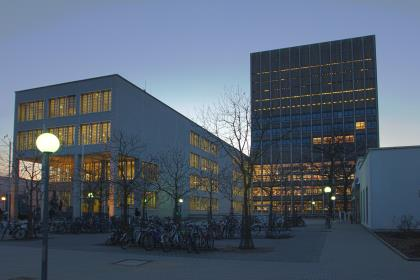
\includegraphics[width=\textwidth]{Figures/bib.jpg}
	\caption{Exterior view of the KIT library. Please always set images manually with the parameter [h]. At this point the image has been placed with the Figure parameter [h]. There is an empty line before and after the Figure environment.}
	\label{fig:bib}
\end{figure}

Lorem ipsum dolor sit amet, consetetur sadipscing elitr, sed diam nonumy eirmod tempor invidunt ut labore et dolore magna aliquyam erat, sed diam voluptua. At vero eos et accusam et justo duo dolores et ea rebum. Stet clita kasd gubergren, no sea takimata sanctus est Lorem ipsum dolor sit amet.

Curabitur a felis in nunc fringilla tristique. Morbi mattis ullamcorper velit. Phasellus gravida semper nisi. Nullam vel sem. Pellentesque libero tortor, tincidunt et, tincidunt eget, semper nec, quam. Sed hendrerit. Morbi ac felis. Nunc egestas, augue at pellentesque laoreet, felis eros vehicula leo, at malesuada velit leo quis pede. Donec interdum, metus et hendrerit aliquet, dolor diam sagittis ligula, eget egestas libero turpis vel mi. Nunc nulla. Fusce risus nisl, viverra et, tempor et.Pellentesque ut neque. Pellentesque habitant morbi tristique senectus et netus et malesuada fames ac turpis egestas. In dui magna, posuere eget, vestibulum et, tempor auctor, justo. In ac felis quis tortor malesuada pretium. Pellentesque auctor neque nec urna. Proin sapien ipsum, porta a, auctor quis, euismod ut, mi.

%\newpage
\begin{figure}[h] % "\begin{figure}" is an environment for floating objects, so that the figure can be numbered and labeled ("\caption{}") and provided with a label ("\label{fig:bib}") and referenced ("\ref{fig:bib} ")
	\centering
	%\hspace{-7pt} % Horizontal shift of the picture row
	\subfloat[Subfloat. Image No. 1. One-line captions are centered.]{%
		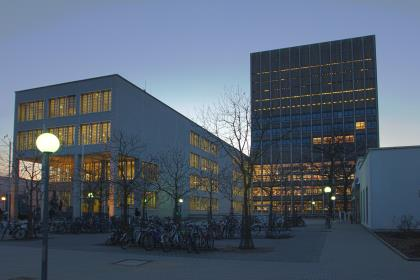
\includegraphics[width=0.49\linewidth]{Figures/bib.jpg}%
	}
	\hfill % Fills the vertical space between the images, provided the images are correspondingly small
	\subfloat[Subfloat. Image No. 2.]{%
		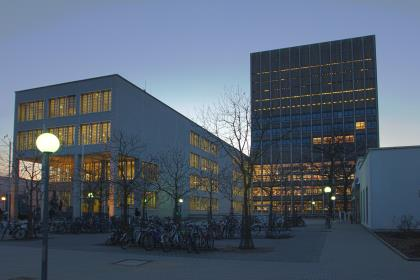
\includegraphics[width=0.49\linewidth]{Figures/bib.jpg}%
	}
	\\ \vspace{3mm} % Distance to the second row of images % plus distance due to the command "\captionsetup[subfloat]{belowskip=}" from the file dokOptions.tex
	%\hspace{-7pt} % Horizontal shift of the picture row
	\subfloat[Subfloat. Image No. 3. Note: If there are only two lines, the caption will not be justified as ragged right when using a manual line break.]{%
		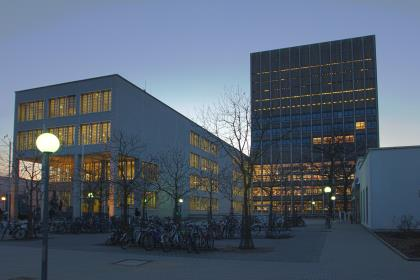
\includegraphics[width=0.49\linewidth]{Figures/bib.jpg}%
	}
	\hfill % Fills the vertical space between the images, provided the images are correspondingly small
	\subfloat[Subfloat. Image No. 4.]{%
		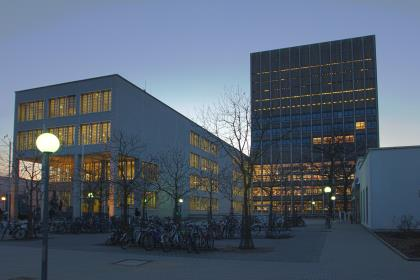
\includegraphics[width=0.49\linewidth]{Figures/bib.jpg}%
	}
	\caption{Exterior view of the KIT library. Please always set images manually with the parameter [h]. This is where the picture has been placed with the Figure parameter [h].}
	\label{fig:bib4}
\end{figure}

Aenean viverra rhoncus pede. Pellentesque habitant morbi tristique senectus et netus et malesuada fames ac turpis egestas. Ut non enim eleifend felis pretium feugiat vivamus quis mi. Phasellus a est. Phasellus magna. In hac habitasse platea dictumst. Curabitur at lacus ac velit ornare lobortis.\footnote{Cabo. Facerfe rferspient que nus molora doleserem. Ut a si autemo tectaquame enihil intota sam am ditati omnihil ma sequis re, aut fugiam earchil luptaque consequ.} Curabitur a felis in nunc fringilla tristique. Morbi mattis ullamcorper velit. Phasellus gravida semper nisi. Nullam vel sem. Pellentesque libero tortor, tincidunt et, tincidunt eget, semper nec, quam. Sed hendrerit.

%\newpage
Pellentesque habitant morbi tristique senectus et netus et malesuada fames ac turpis egestas. In dui magna, posuere eget, vestibulum et, tempor auctor, justo. In ac felis quis tortor malesuada pretium. Pellentesque auctor neque nec urna. Proin sapien ipsum, porta a, auctor quis, euismod ut, mi. Aenean viverra rhoncus pede. Pellentesque habitant morbi tristique senectus et netus et malesuada fames ac turpis egestas. Ut non enim eleifend felis pretium feugiat vivamus quis mi. Phasellus a est. Phasellus magna. In hac habitasse platea dictumst. Curabitur at lacus ac velit ornare lobortis. Aenean viverra rhoncus pede. Pellentesque habitant morbi tristique senectus et netus et malesuada fames ac turpis egestas. Ut non enim eleifend felis pretium feugiat vivamus quis mi. Phasellus a est. Phasellus magna. Phasellus a est. Phasellus magna. In hac habitasse platea dictumst. Curabitur at lacus ac velit ornare lobortis. Aenean viverra rhoncus pede. Pellentesque habitant morbi tristique senectus et netus et malesuada fames ac turpis egestas. Ut non enim eleifend felis pretium feugiat vivamus quis mi. Phasellus a est. Phasellus magna.

Phasellus magna. Phasellus a est. Phasellus magna. In hac habitasse platea dictumst. Curabitur at lacus ac velit ornare lobortis. Aenean viverra rhoncus pede. Pellentesque habitant morbi tristique senectus et netus et malesuada fames ac turpis egestas. Ut non enim eleifend felis pretium feugiat vivamus quis mi. Phasellus a est. Phasellus magna et netus et malesuada fames ac turpis egestas.

%\newpage
\begin{figure}[h]
	\centering
	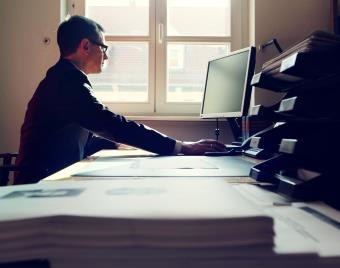
\includegraphics[width=6cm]{Figures/knowledge.jpg}
	\caption[Scientist in his workplace.] {Scientist in his workplace. Please always set images manually with the parameter [h]. At this point the image has been placed with the Figure parameter [h]. There is an empty line before and after the figure environment.}
	\label{fig:knowledge}
\end{figure}

Pellentesque habitant morbi tristique senectus et netus et malesuada fames ac turpis egestas. In dui magna, posuere eget, vestibulum et, tempor auctor, justo. In ac felis quis tortor malesuada pretium. Pellentesque auctor neque nec urna. Proin sapien ipsum, porta a, auctor quis, euismod ut, mi. Aenean viverra rhoncus pede. Pellentesque habitant morbi tristique senectus et netus et malesuada fames ac turpis egestas. Ut non enim eleifend felis pretium feugiat vivamus quis mi. Phasellus a est. Phasellus magna. In hac habitasse platea dictumst. Curabitur at lacus ac velit ornare lobortis.

Pellentesque habitant morbi tristique senectus et netus et malesuada fames ac turpis egestas. In dui magna, posuere eget, vestibulum et, tempor auctor, justo. In ac felis quis tortor malesuada pretium. Pellentesque auctor neque nec urna. Proin sapien ipsum, porta a, auctor quis, euismod ut, mi. Aenean viverra rhoncus pede. Pellentesque habitant morbi tristique senectus et netus et malesuada fames ac turpis egestas. Ut non enim eleifend felis pretium feugiat vivamus quis mi. Phasellus a est. Phasellus magna. In hac habitasse platea dictumst. Curabitur at lacus ac velit ornare lobortis. Pellentesque habitant morbi tristique senectus et netus et malesuada fames ac turpis egestas.

%Pellentesque habitant morbi tristique senectus et netus et malesuada fames ac turpis egestas. In dui magna, posuere eget, vestibulum et, tempor auctor. Pellentesque habitant morbi tristique senectus et netus et malesuada fames ac turpis egestas. In dui magna, posuere eget, vestibulum et, tempor auctor.

\begin{table}[h] % "\ begin {table}" is an environment for floating objects, so that the table "\ begin {tabular}" can be numbered, titled, labeled and referenced
	\caption{Tables are always inserted with the parameter [h].}
	\begin{tabularx}{\textwidth}{XXXXXXXX} \toprule
		Spalte1 & Spalte2 & Spalte3 & Spalte4 & Spalte5
		& Spalte6 & Spalte7 & Spalte8 \\ \midrule
		AA      & BB      & CC      & DD      &
		EE      & FF      & GG      & HH       \\
		AA      & BB      & CC      & DD
		& EE      & FF      & GG      & HH    \\
		AA      & BB      & CC      & DD
		& EE      & FF      & GG      & HH    \\
		AA      & BB      & CC      & DD
		& EE      & FF      & GG      & HH    \\
		AA      & BB      & CC      & DD
		& EE      & FF      & GG      & HH    \\
		AA      & BB      & CC      & DD
		& EE      & FF      & GG      & HH     \\ \bottomrule
	\end{tabularx}
\end{table}

Pellentesque habitant morbi tristique senectus et netus et malesuada fames ac turpis egestas. In dui magna, posuere eget, vestibulum et, tempor auctor. Pellentesque habitant morbi tristique senectus et netus et malesuada fames ac turpis egestas. In dui magna, posuere eget, vestibulum et, tempor auctor.

% Theory
\markboth{Theory}{Theory}
\chapter[Theory (here is the short title in the table of contents and in the header)]{Theory. Here is the long title in the body text for the Header would be too long or run over two lines. Breaks in headlines can generated with mbox}
\label{cha:Theory}

%%%%%%%%%%%%%%%%%%%%%%%%%%%%%%%%%%%%%%%%%%%%%%%%%%

Lorem ipsum dolor sit amet, consetetur sadipscing elitr, sed diam nonumy eirmod tempor invidunt ut labore et dolore magna aliquyam erat, sed diam voluptua. At vero eos et accusam et justo duo dolores et ea rebum. Stet clita kasd gubergren, no sea takimata sanctus est Lorem ipsum dolor sit amet. Lorem ipsum dolor sit amet, consetetur sadipscing elitr, sed diam nonumy eirmod tempor invidunt ut labore et dolore magna aliquyam erat, sed diam voluptua. At vero eos et accusam et justo duo dolores et ea rebum. Stet clita kasd gubergren, no sea takimata sanctus est Lorem ipsum dolor sit amet.

Lorem ipsum dolor sit amet, consetetur sadipscing elitr, sed diam nonumy eirmod tempor invidunt ut labore et dolore magna aliquyam erat, sed diam voluptua. At vero eos et accusam et justo duo dolores et ea rebum. Stet clita kasd gubergren, no sea takimata sanctus est Lorem ipsum dolor sit amet. Lorem ipsum dolor sit amet, consetetur sadipscing elitr, sed diam nonumy eirmod tempor invidunt ut labore et dolore magna aliquyam erat, sed diam voluptua. At vero eos et accusam et justo duo dolores et ea rebum. Stet clita kasd gubergren, no sea takimata sanctus est Lorem ipsum dolor sit amet.

Lorem ipsum dolor sit amet, consetetur sadipscing elitr, sed diam nonumy eirmod tempor invidunt ut labore et dolore magna aliquyam erat, sed diam voluptua. At vero eos et accusam et justo duo dolores et ea rebum. Stet clita kasd gubergren, no sea takimata sanctus est Lorem ipsum dolor sit amet. Lorem ipsum dolor sit amet, consetetur sadipscing elitr, sed diam nonumy eirmod tempor invidunt ut labore et dolore magna aliquyam erat, sed diam voluptua. At vero eos et accusam et justo duo dolores et ea rebum. Stet clita kasd gubergren, no sea takimata sanctus est Lorem ipsum dolor sit amet.

\begin{table}[h] % "\ begin {table}" is an environment for floating objects, so that the table "\ begin {tabular}" can be numbered, titled, labeled and referenced
	\caption[Od quo tecto offic torit eteum acerum fuga. Ideni omnihic idundero doluptus iminvel luptati busdaepta sequi dolorec tatessinum.]{Tables are also always inserted with the parameter [h]. There is an empty line before and after the table environment. Use the command ``\textbackslash newline'' to insert manual line breaks if the spacing between words in a cell becomes too large.}
	\centering
	\begin{tabular}{ | l | l | l | p{2.5cm} |}
			\hline
			Aliquyam & Dolor & Rebum & Sadipscing \\ \hline
			Invidunt & Labore & Sanctus & Stet clita kasd \newline gubergren. \\ \hline
			Magna & Gubergren & Clita & No sea takimata \newline sanctus. \\ \hline
			Eirmod & Voluptua & Aliquyam & Sed diam nonumy eirmod tempor. \\
			\hline
	\end{tabular}
	\label{tab:tab}
\end{table}

Od quo tecto offic torit eteum acerum fuga. Ideni omnihic idundero doluptus iminvel luptati busdaepta sequi dolorec tatessinum quas et quia perae et qui blanditi quiberit alique provit, cus incipid ut quis enis vel id es asperum volor aut unt, quatum eturem aciassin et rest inulluptam et volecae. Od quo tecto offic torit eteum acerum fuga. Ideni omnihic idundero doluptus iminvel luptati busdaepta sequi dolorec tatessinum quas et quia perae et qui blanditi quiberit alique provit, cus incipid ut quis enis vel id es asperum volor aut unt, quatum eturem aciassin et rest inulluptam et volecae. Od quo tecto offic torit eteum acerum fuga. Ideni omnihic idundero doluptus iminvel luptati busdaepta sequi dolorec tatessinum quas et quia perae et qui blanditi quiberit alique provit, cus incipid ut quis enis vel id es asperum volor aut unt, quatum eturem aciassin et rest inulluptam et volecae. Od quo tecto offic torit eteum acerum fuga. Ideni omnihic idundero doluptus iminvel luptati busdaepta sequi dolorec tatessinum quas et quia perae et qui blanditi quiberit alique provit, cus incipid ut quis enis vel id es asperum volor aut unt, quatum eturem aciassin et rest inulluptam et volecae.
\begin{subequations}
	\label{maxwell-gleichungen}
	\begin{align}
	\text{div }(\vec{D}) &= 4 \cdot \pi \cdot \rho
	\label{coulomb-gesetz}\\
	\text{rot }(\vec{H}) &= \frac{4 \cdot \pi}{c} \cdot \vec{j}
	\label{ampere-gesetz}\\
	\text{rot }(\vec{E}) &= - \frac{1}{c} \cdot \frac{\partial \vec{B}}{\partial t}
	\label{faraday-gesetz-1} \\
	\text{div }(\vec{B}) &= 0
	\label{faraday-gesetz-2}
	\end{align}
\end{subequations}
Arepelisti re denda doluptata quo demque conseribeate eum quiberor aut quatur maiorae riberis eserio eaturepro ommo bero eum que quisquidit volendis eni asi sint aut pe minis is re nonseque ius aut pa is expel ium nobis miliquati dolupit, qui nullanis re, sitiis si volor mo te eventia vendit qui dolupta quamusda vereped magnihi cturem dendignatus vite prernatatis soluptat aperum sequostorum et quistru pienitiis arum, optaquo qui comnis cuptam qui officitate pellent ariae occaborrovid mod esequi dolorum rerro quas vent harciistia quis voloris sinctiis ea nistrum facius simus utem sit, inctor sit dolorrum ditio. Ecerum et est quia doluptur? Qui dolorero des nosapis exerias dest, qui coratur itemporum repeliq uiassit, inum fugiasi simil est alicium ilis que nimusanis es suntiaestrum ium ium harcil iligent excearum fugia nonsequia dem.
% Binomial coefficient:
\begin{align*}
\binom{n}{k} = \frac{n!}{(n - k)! \cdot k!}
\end{align*}
Optaquo qui comnis cuptam qui officitate pellent ariae occaborrovid mod esequi dolorum rerro quas vent harciistia quis voloris sinctiis ea nistrum facius simus utem sit, inctor sit dolorrum ditio. Ecerum et est quia doluptur? Qui dolorero des nosapis exerias dest, qui coratur itemporum repeliq uiassit, inum fugiasi simil est alicium ilis que nimusanis es suntiaestrum ium ium harcil iligent excearum fugia nonsequia dem.
\begin{equation} 
\prod \limits_{i=1}^{n+1}i = 1\cdot 2\cdot\dots\cdot n\cdot (n+1) \
\end{equation}
Arepelisti re denda doluptata quo demque conseribeate eum quiberor aut quatur maiorae riberis eserio eaturepro ommo bero eum que quisquidit volendis eni asi sint aut pe minis is re nonseque ius aut pa is expel ium nobis miliquati dolupit, qui nullanis re, sitiis si volor mo te eventia vendit qui dolupta quamusda vereped magnihi cturem dendignatus vite prernatatis soluptat aperum sequostorum et quistru pienitiis arum, optaquo qui comnis cuptam qui officitate pellent ariae occaborrovid mod esequi dolorum rerro quas vent harciistia quis voloris sinctiis ea nistrum facius simus utem sit, inctor sit dolorrum ditio. Ecerum et est quia doluptur? Qui dolorero des nosapis exerias dest, qui coratur itemporum repeliq uiassit, inum fugiasi simil est alicium ilis que nimusanis es suntiaestrum ium ium harcil iligent excearum fugia nonsequia dem. Ovidus.

% Headlines
% \chapter{Überschriften}

% Stehen zwei Überschriften direkt untereinander, muss die Autorin oder der Autor zwischen den Überschriften manuell eine Anpassung des vertikalen Abstands mit dem Befehl \glqq vspace\grqq{} vornehmen. Für die folgende Aneinanderreihung der Überschriften entnehmen Sie den vertikalen Abstand bitte wie folgt:

% \begin{itemize}

% \item \raggedright Zwischen \glqq chapter\grqq{} und \glqq section\grqq{} bitte mit dem Befehl \glqq vspace\grqq{} einen zusätzlichen vertikalen Abstand einfügen von \hbox{-}3~mm. 
% \begin{Verbatim}
% \chapter{Überschrift Ebene Chapter}
% \vspace{-3mm}
% \section{Überschrift Ebene Section}
% \end{Verbatim}
% (Sollabstand: 10~mm, gemessen von der Grundlinie der Überschrift \glqq chapter\grqq{} zur H-Linie der Überschrift \glqq section\grqq{}) 

% \item \raggedright Zwischen \glqq section\grqq{} und \glqq subsection\grqq{} bitte mit dem Befehl \glqq vspace\grqq{} einen zusätzlichen vertikalen Abstand einfügen von 2~mm. 
% \begin{Verbatim}
% \section{Überschrift Ebene Section}
% \vspace{2mm}
% \subsection{Überschrift Ebene Subsection}
% \end{Verbatim}
% (Sollabstand: 10~mm, gemessen von der Grundlinie der Überschrift \glqq section\grqq{} zur H-Linie der Überschrift \glqq subsection\grqq{})

% \item \raggedright Zwischen \glqq subsection\grqq{} und \glqq subsubsection\grqq{} bitte mit dem Befehl \glqq vspace\grqq{} einen zusätzlichen vertikalen Abstand einfügen von 3~mm. 
% \begin{Verbatim}
% \subsection{Überschrift Ebene Subsection}
% \vspace{3mm}
% \subsubsection{Überschrift Ebene Subsubsection}
% \end{Verbatim}
% (Sollabstand: 10~mm, gemessen von der Grundlinie der Überschrift \glqq subsection\grqq{} zur H-Linie der Überschrift \glqq subsubsection\grqq{}. 

% \end{itemize}

% % Für die exakte Angabe des Befehls \glqq vspace\grqq{} mit den entsprechenden Werten sehen Sie bitte in die Datei \glqq content\_vorlage/ueberschriften.tex\grqq{}. 
% Das Ergebnis mit den entsprechenden vertikalen Abständen zwischen den Überschriften sehen Sie in Kapitel \ref{chap:UeberschriftenEbenen} (\glqq \nameref{chap:UeberschriftenEbenen}\grqq{}) auf Seite \pageref{chap:UeberschriftenEbenen} in dieser PDF-Datei.



\chapter{Headline level 1 (chapter)}
\label{chap:HeadlinesLevel}
% Lorem ipsum dolor sit amet, consectetuer adipiscing elit. Aenean co~mmodo ligula eget dolor. Aenean massa.
% \vspace{-3mm} % Folgt kein Text nach der Überschrift, muss der Abstand zur nächsten Überschrift manuell angepasst werden

\section{Headline level 2 (section)}
% Lorem ipsum dolor sit amet, consectetuer adipiscing elit. Aenean co~mmodo ligula eget dolor. Aenean massa.
\vspace{1.5mm} % Folgt kein Text nach der Überschrift, muss der Abstand zur nächsten Überschrift manuell angepasst werden 

\subsection{Headline level 3 (subsection)}
% Lorem ipsum dolor sit amet, consectetuer adipiscing elit. Aenean co~mmodo ligula eget dolor. Aenean massa.
\vspace{3mm} % Folgt kein Text nach der Überschrift, muss der Abstand zur nächsten Überschrift manuell angepasst werden

\subsubsection{Headline level 4 (subsubsection)}
% Lorem ipsum dolor sit amet, consectetuer adipiscing elit. Aenean co~mmodo ligula eget dolor. Aenean massa.


% Summary and outlook
\markboth{Summary}{Summary}
\chapter{Summary}
\label{cha:Summary}

%%%%%%%%%%%%%%%%%%%%%%%%%%%%%%%%%%%%%%%%%%%%%%%%%%

\section{Summary}
\label{sec:Summary}
Arepelisti re denda doluptata quo demque conseribeate eum quiberor aut quatur maiorae riberis eserio eaturepro ommo bero eum que quisquidit volendis eni asi sint aut pe minis is re nonseque ius aut pa is expel ium nobis miliquati dolupit, qui nullanis re, sitiis si volor mo te eventia vendit qui dolupta quamusda vereped magnihi cturem dendignatus vite prernatatis soluptat aperum sequostorum et quistru pienitiis arum, optaquo qui comnis cuptam qui officitate pellent ariae occaborrovid mod esequi dolorum rerro quas vent harciistia quis voloris sinctiis ea nistrum facius simus utem sit, inctor sit dolorrum ditio. Ecerum et est quia doluptur? Qui dolorero des nosapis exerias dest, qui coratur itemporum repeliq uiassit, inum fugiasi simil est alicium ilis que nimusanis es suntiaestrum ium ium harcil iligent excearum fugia nonsequia dem.

Arepelisti re denda doluptata quo demque conseribeate eum quiberor aut quatur maiorae riberis eserio eaturepro ommo bero eum que quisquidit volendis eni asi sint aut pe minis is re nonseque ius aut pa is expel ium nobis miliquati dolupit, qui nullanis re, sitiis si volor mo te eventia vendit qui dolupta quamusda vereped magnihi cturem dendignatus vite prernatatis soluptat aperum sequostorum et quistru pienitiis arum, optaquo qui comnis cuptam qui officitate pellent ariae occaborrovid mod esequi dolorum rerro quas vent harciistia quis voloris sinctiis ea nistrum facius simus utem sit, inctor sit dolorrum ditio. Ecerum et est quia doluptur? Qui dolorero des nosapis exerias dest, qui coratur itemporum repeliq uiassit, inum fugiasi simil est alicium ilis que nimusanis es suntiaestrum ium ium harcil iligent excearum fugia nonsequia dem.

\section{Outlook}
\label{sec:Outlook}
Arepelisti re denda doluptata quo demque conseribeate eum quiberor aut quatur maiorae riberis eserio eaturepro ommo bero eum que quisquidit volendis eni asi sint aut pe minis is re nonseque ius aut pa is expel ium nobis miliquati dolupit, qui nullanis re, sitiis si volor mo te eventia vendit qui dolupta quamusda vereped magnihi cturem dendignatus vite prernatatis soluptat aperum sequostorum et quistru pienitiis arum, optaquo qui comnis cuptam qui officitate pellent ariae occaborrovid mod esequi dolorum rerro quas vent harciistia quis voloris sinctiis ea nistrum facius simus utem sit, inctor sit dolorrum ditio. Ecerum et est quia doluptur? Qui dolorero des nosapis exerias dest, qui coratur itemporum repeliq uiassit, inum fugiasi simil est alicium ilis que nimusanis es suntiaestrum ium ium harcil iligent excearum fugia nonsequia dem.



%%%%%%%%%%%%%%%%%%%%%%%%%%%%%%%%%%%%%%%%%%%%%%%%%%
%%%				Appendix (include!)	 		             %%%
%%%%%%%%%%%%%%%%%%%%%%%%%%%%%%%%%%%%%%%%%%%%%%%%%%

% Appendix; chapters in the appendix receive capital letters in the table of contents
\appendix 

\markboth{Appendix}{Appendix}
\chapter{Appendix}
\label{cha:Appendix}

%%%%%%%%%%%%%%%%%%%%%%%%%%%%%%%%%%%%%%%%%%%%%%%%%%

Lorem ipsum dolor sit amet, consetetur sadipscing elitr, sed diam nonumy eirmod tempor invidunt ut labore et dolore magna aliquyam erat, sed diam voluptua. At vero eos et accusam et justo duo dolores et ea rebum. Stet clita kasd gubergren, no sea takimata sanctus est Lorem ipsum dolor sit amet. Lorem ipsum dolor sit amet, consetetur sadipscing elitr, sed diam nonumy eirmod tempor invidunt ut labore et dolore magna aliquyam erat, sed diam voluptua. At vero eos et accusam et justo duo dolores et ea rebum. Stet clita kasd gubergren, no sea takimata sanctus est Lorem ipsum dolor sit amet.

%%%%%%%%%%%%%%%%%%%%%%%%%%%%%%%%%%%%%%%%%%%%%%%%%%
%%%				List of (include!)			             %%%
%%%%%%%%%%%%%%%%%%%%%%%%%%%%%%%%%%%%%%%%%%%%%%%%%%

% List of figures
\listoffigures

% List of tables
\listoftables

% Listings
\renewcommand{\lstlistlistingname}{\latex source code} % Changes the headline and bookmark in the PDF file from "List" to "LaTeX source code"; this command must be placed here
% \lstlistoflistings

% Bibliography
\markboth{Bibliography}{Bibliography}

%%%%%%%%%%%%%%%%%%%%%%%%%%%%%%%%%%%%%%%%%%%%%%%%%%

\chapter*{List of Publications}
\addcontentsline{toc}{chapter}{List of Publications}

\section*{Journal articles}
\addcontentsline{toc}{section}{Journal articles}
\renewcommand{\refnamejournal}{Journal articles}
\begingroup % Delete heading from \ bibliography {}
\renewcommand{\chapter}[2]{}
\renewcommand{\section}[2]{}
\nocitejournal{*} % Show all titles of the .bib file in the bibliography, if activated; if deactivated, only the quoted titles are displayed
\bibliographystylejournal{plainnat}
\bibliographyjournal{Bibliography/Own_journal_papers}{}
\endgroup

%%%%%%%%%%%%%%%%%%%%%%%%%%%%%%%%%%%%%%%%%%%%%%%%%%

\section*{Conference contributions}
\addcontentsline{toc}{section}{Conference contributions}
\renewcommand{\refnameconference}{Conference contributions}
\begingroup % Delete heading from \ bibliography {}
\renewcommand{\chapter}[2]{}
\renewcommand{\section}[2]{}
\nociteconference{*} % Show all titles of the .bib file in the bibliography, if activated; if deactivated, only the quoted titles are displayed
\bibliographystyleconference{plainnat}
\bibliographyconference{Bibliography/Own_conference_papers}{}
\endgroup

%%%%%%%%%%%%%%%%%%%%%%%%%%%%%%%%%%%%%%%%%%%%%%%%%%

\chapter*{Bibliography}
\addcontentsline{toc}{chapter}{Bibliography}
%\renewcommand{\refname}{Literaturverzeichnis}
%\renewcommand\bibname{Literaturverzeichnis}
\begingroup % Überschrift von \bibliography{} löschen
\renewcommand{\chapter}[2]{}
\renewcommand{\section}[2]{}
\nocite{*} % Show all titles of the .bib file in the bibliography, if activated; if deactivated, only the quoted titles are displayed
\bibliographystyle{plainnat} % Adjust the citation style if necessary
\bibliography{Bibliography/Literature}{}
\endgroup

%%%%%%%%%%%%%%%%%%%%%%%%%%%%%%%%%%%%%%%%%%%%%%%%%%

%\markboth{Literaturverzeichnis}{Literaturverzeichnis}
%\renewcommand{\refname}{Literaturverzeichnis}
%\renewcommand\bibname{Literaturverzeichnis}
%\bibliography{Literatur/Eigene_Konferenz_Papers}{}
%\bibliographystyle{alpha}
%\nocite{*}

\end{document}